\section{Event Selection}


\begin{frame}{Analysis workflow}
  \begin{center}
  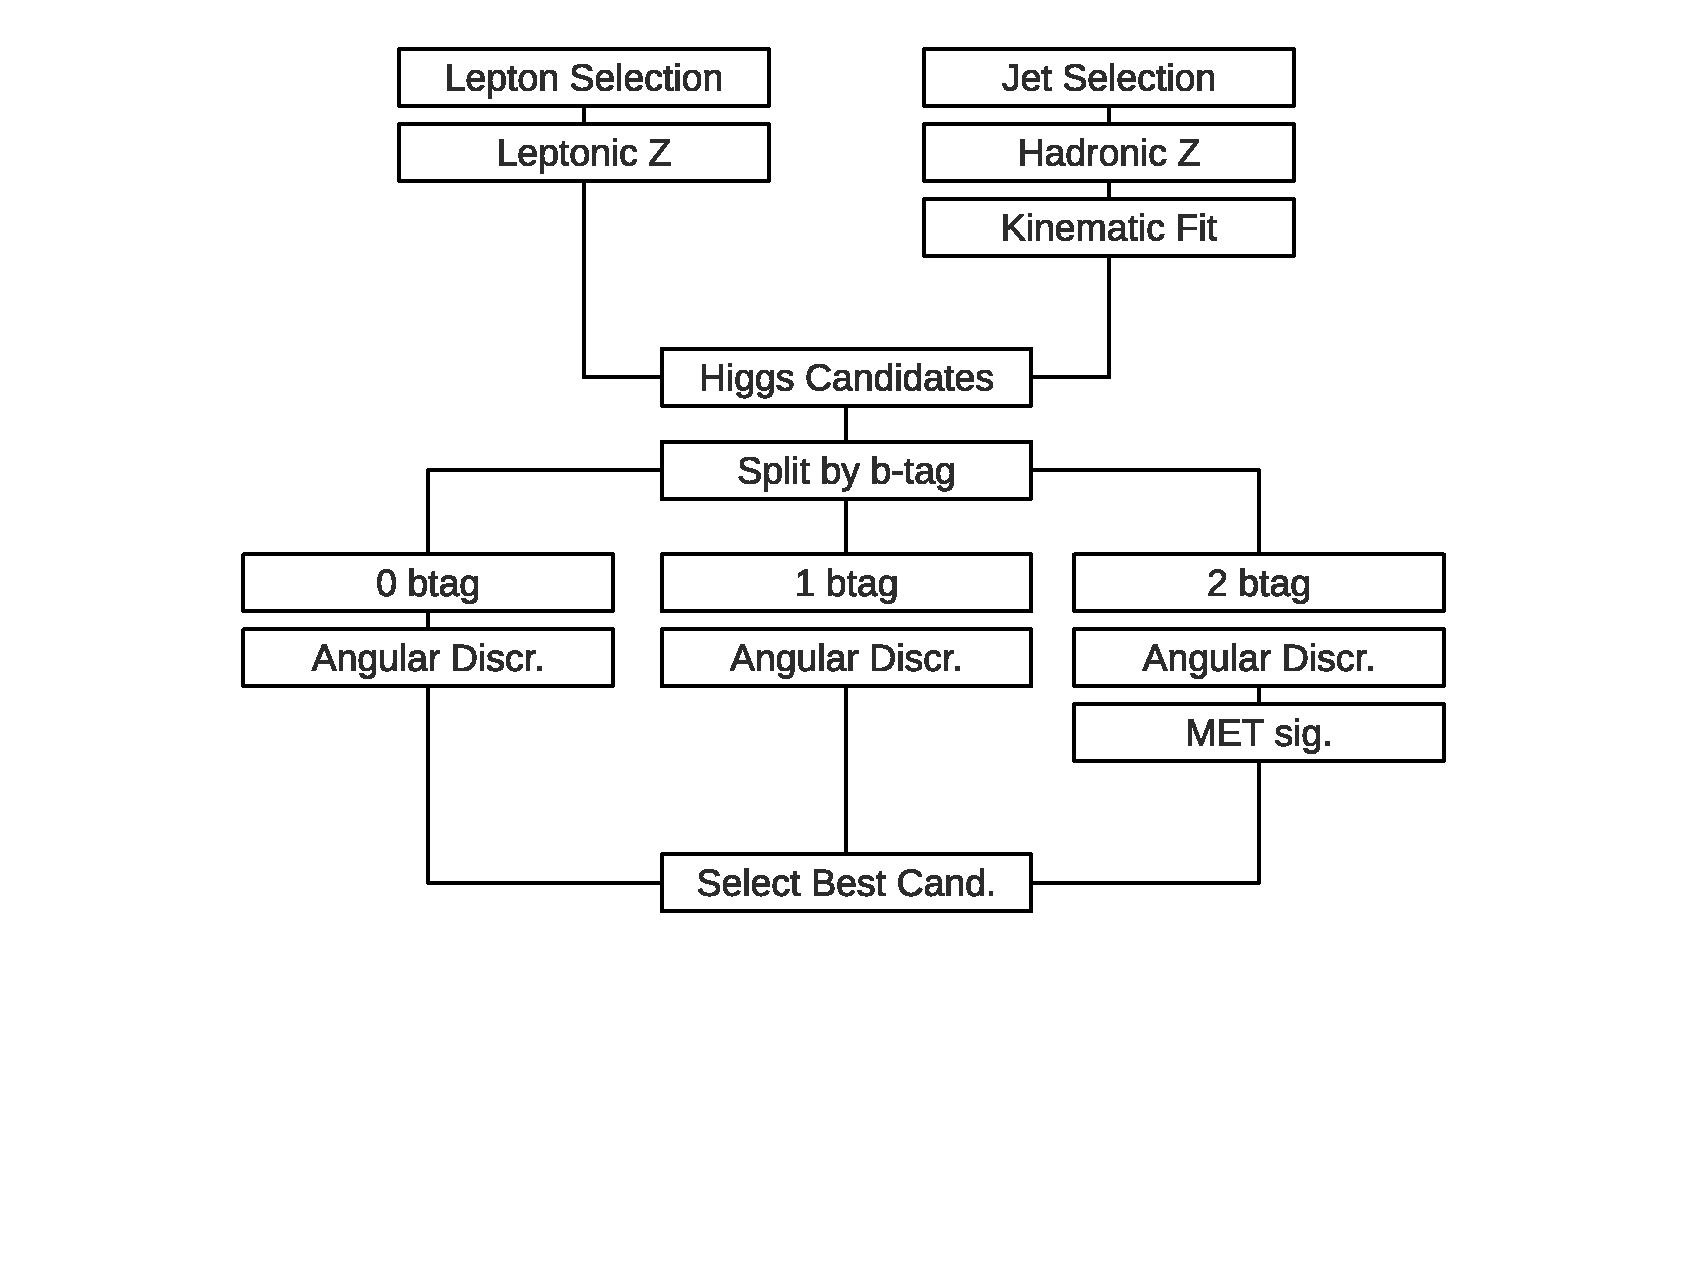
\includegraphics[width=1.0\textwidth]{images/workflow.eps}
  \end{center}
\end{frame}


\begin{frame}{Samples}
%  \begin{itemize}
%  \item
%    Data is Double Electron and Double Muon datasets.
%  \item
%    Background Monte Carlo is primaraly Z+Jets make with the MADGRAPH.
%  \item
%    Other Backgrounds are TT, WW, WZ, ZZ with PYTHIA.
%  \item
%    The signal Monte Carlo samples are POWHEG.
%  \end{itemize}

\begin{center}

Data is Double Electron and Double Muon datasets.\\
\vspace{2em}
Background\\
\begin{tabular}{|c|c|c|}\hline
  MC Sample & Generator & Percent of Final Region \\ \hline \hline
  Z+Jets  & MADGRAPH & 80\% \\ \hline 
    tt      & PYTHIA & 7\%  \\ \hline
    ZZ      & PYTHIA & 11\% \\ \hline
    WZ      & PYTHIA & 2\%  \\ \hline
    WW      & PYTHIA & <1\% \\ \hline
\end{tabular}
\\
\vspace{2em}
The signal Monte Carlo samples are POWHEG.

$m_{H} = $200,210,220,230,250,275,300,325,\\
350,375,400,425,450,475,500,525,550,575,600 GeV

\end{center}

\end{frame}



\begin{frame}{Leptons}
  We are using the official prescriptions from the POGs for both Lepton ID and Isolation.
%\vspace{1em}
\begin{columns}
      \begin{column}{0.5\textwidth}
        \begin{center}
  {\bf Electrons}
  \begin{itemize}
    \footnotesize
  \item
    GSF Elecrons
  \item
    $p_{T}$ > 40/20 GeV, $|\eta|$ < 2.5
  \item
    Working Point Loose
  \item
    + Tight trigger cuts
  \item
    PU corrected ISO < 0.15
  \end{itemize}
  \vspace{2em}

  {\bf Muons}
  \begin{itemize}
    \footnotesize
    %\scriptsize
  \item
    reco::Muons
  \item
    $p_{T}$ > 40/20 GeV, $|\eta|$ < 2.4
  \item
    Tight Muon
  \item
    PU corrected ISO < 0.12
  \end{itemize}
  \end{center}
\end{column}
      
      \begin{column}{0.5\textwidth}
        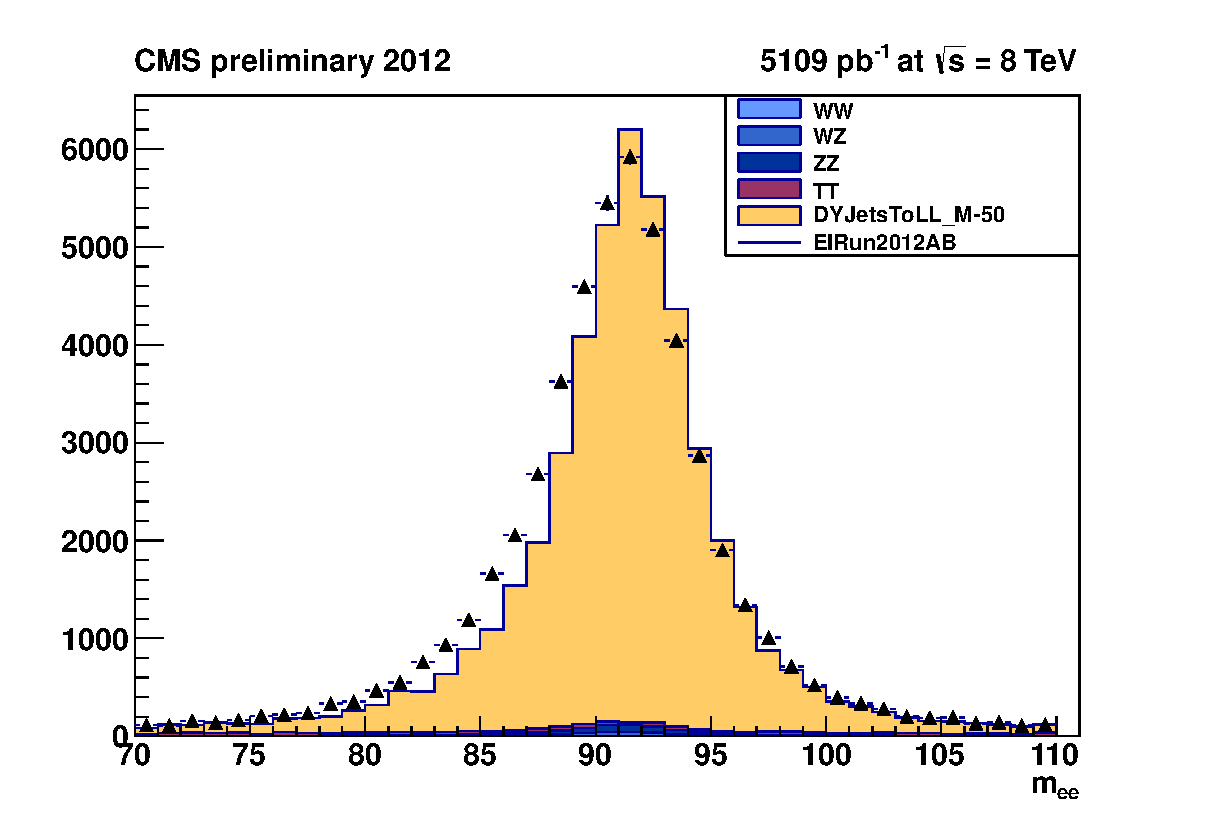
\includegraphics[width=0.8\textwidth]{images/stdCandle_ElRun2012.eps}\\
         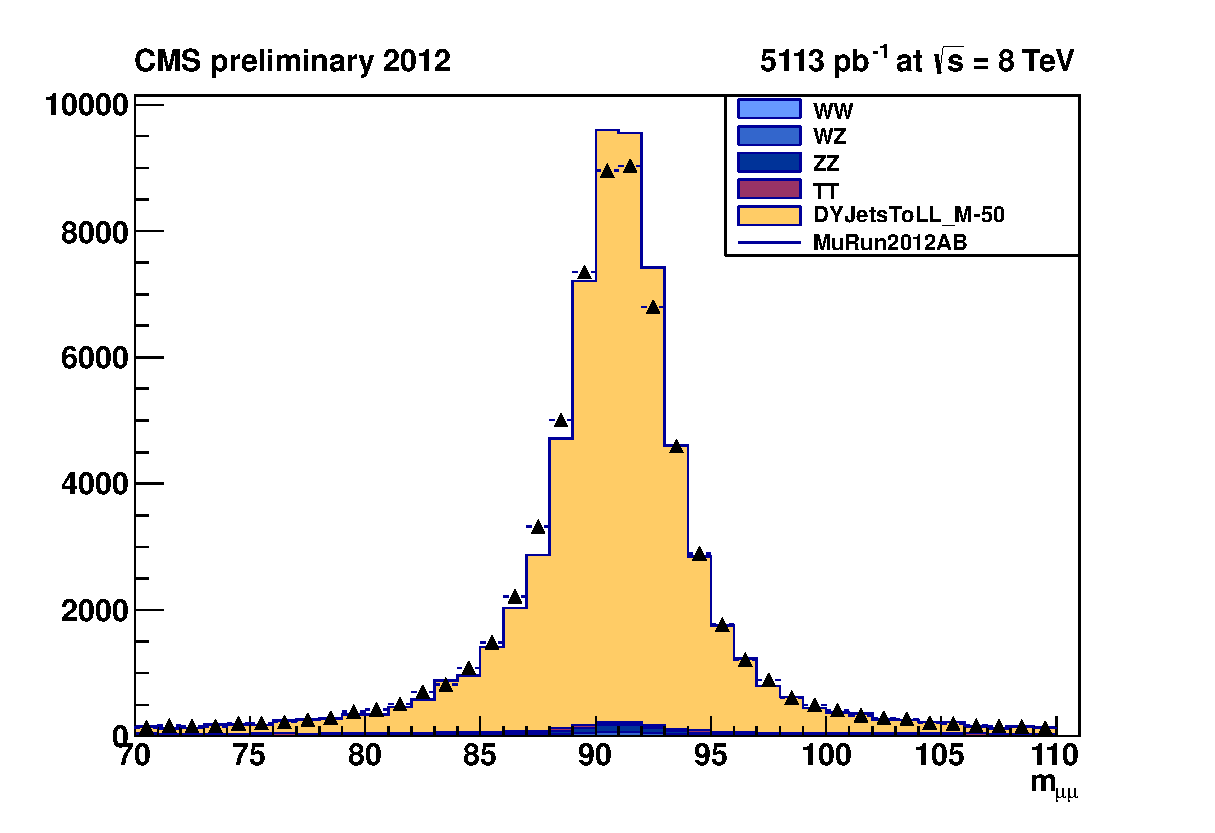
\includegraphics[width=0.8\textwidth]{images/stdCandle_MuRun2012.eps}
\end{column}
\end{columns}
\end{frame}




\begin{frame}{Jets}
  
      \begin{itemize}
      \item
        AK5PF, L1FastJet+L2+L3  %no MVA ID applied
      \item
        p$_{T}$ > 30 GeV , $|\eta|$ < 2.4
      \end{itemize}

  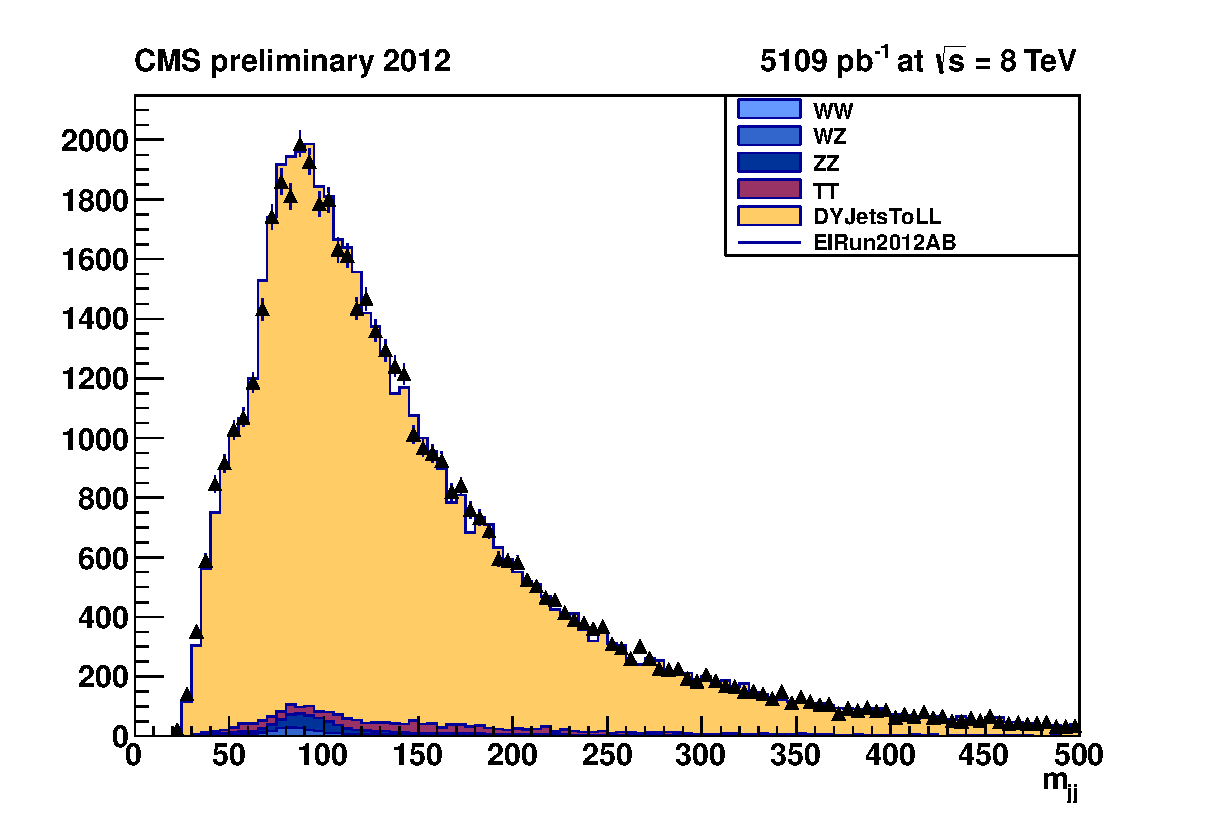
\includegraphics[width=0.5\textwidth]{images/zjjmass_ElRun2012.eps}
  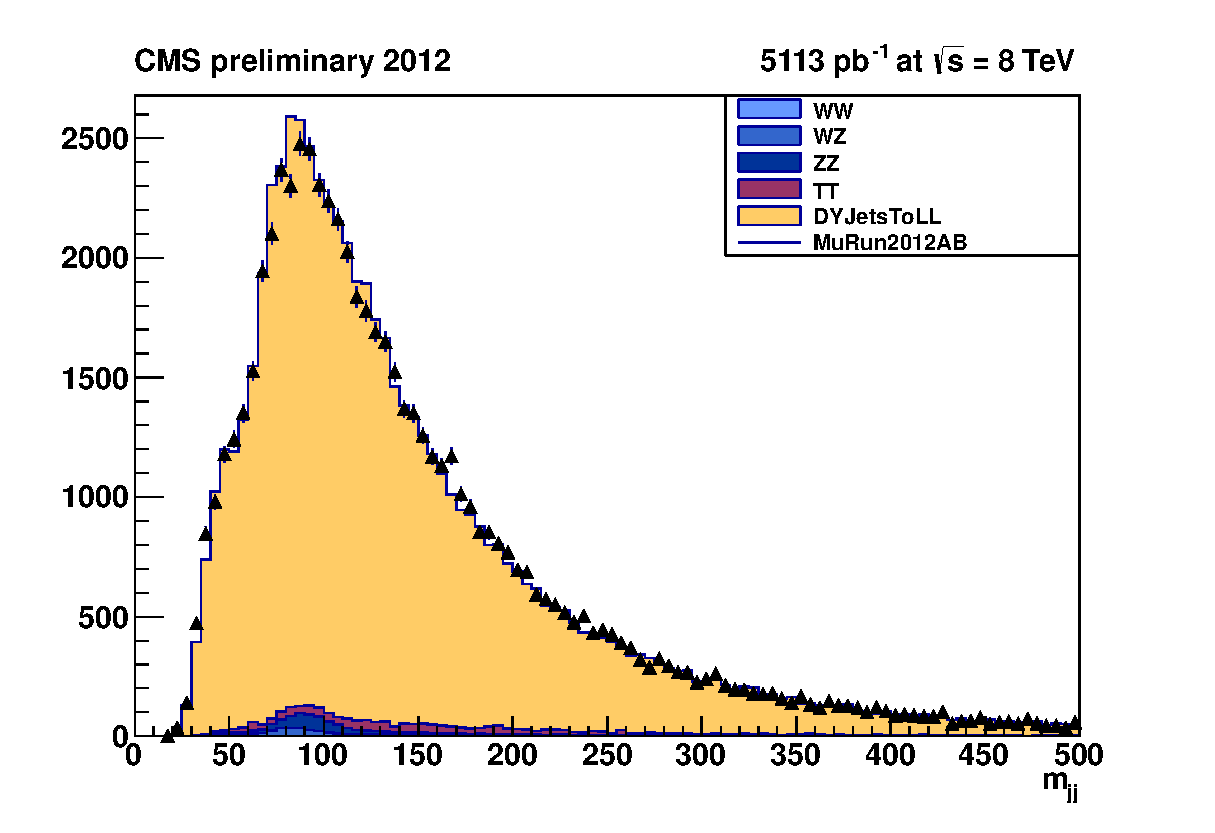
\includegraphics[width=0.5\textwidth]{images/zjjmass_MuRun2012.eps}

\end{frame}
















\begin{frame}{$b$-tagging}
  \begin{columns}
    \begin{column}{0.4\textwidth}
      \begin{itemize}
        {\small
        \item Using {\bf JP algorithm}, ``loose'' and ``medium'' WPs, allowing migrations among the tagging categories when applying the SF to MC
        \item Up to date using the latest calibrations available for the JP algorithm
        }
      \end{itemize}
      
    \end{column}
    
    \begin{column}{0.6\textwidth}
      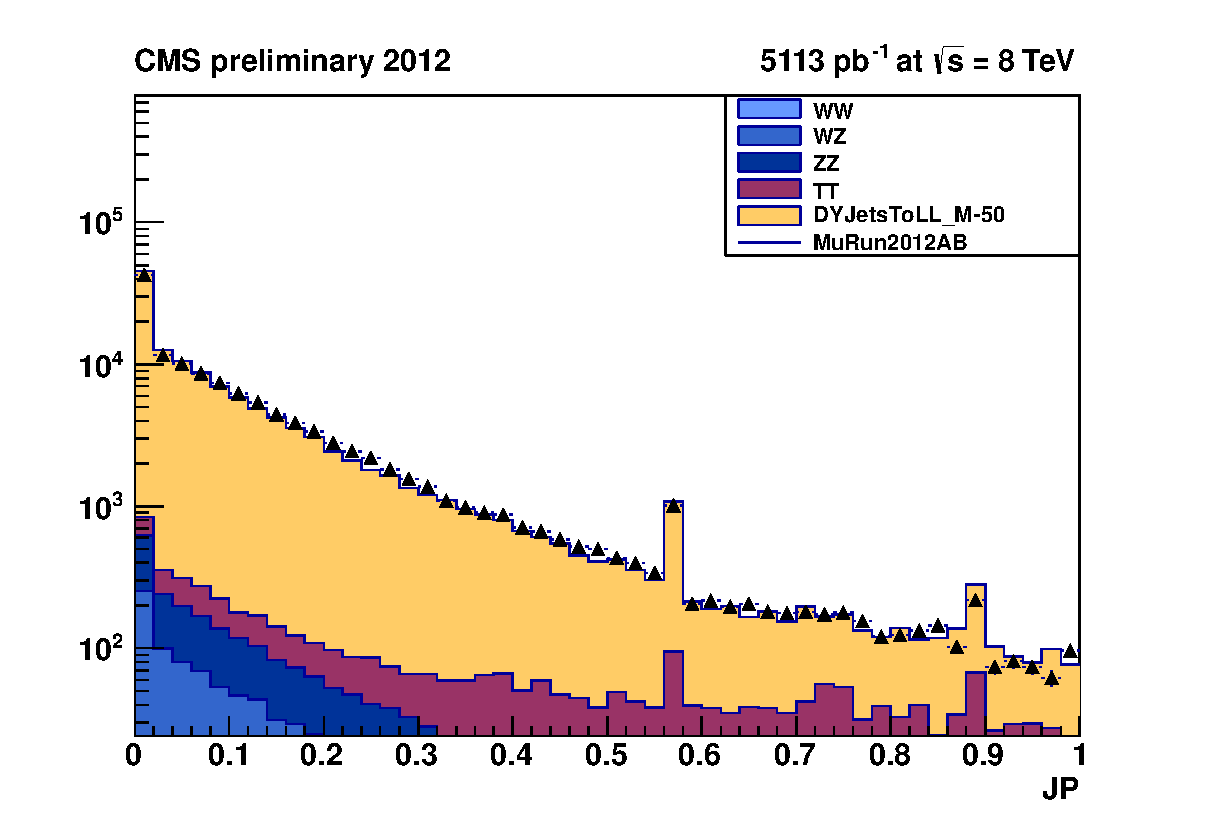
\includegraphics[width=0.99\textwidth]{images/JPJet_MuRun2012_LOG.eps}
    \end{column}
  \end{columns}
 \begin{center}
  \begin{tabular}{|c|c|}\hline
    0 - tag  & Both Jets < Loose \\ \hline 
    1 - tag  & > Loose and < Medium \\ \hline
    2 - tag  & > Loose and > Medium \\ \hline
  \end{tabular}
  \end{center}
\end{frame}



\begin{frame}{Signal and Sideband Regions}
  {\bf Study Regions}
  \begin{itemize}
  \item 
   Signal Region is 70 < m$_{ll}$ < 110 GeV and 75 < m$_{jj}$ < 105 GeV
  \item 
    Also we are looking at the sidebands region, defined as 60< m$_{jj}$ <75 GeV || 105< m$_{jj}$ <130 GeV (i.e. outside signal window 75< mjj < 105 GeV).
  \end{itemize}
 % 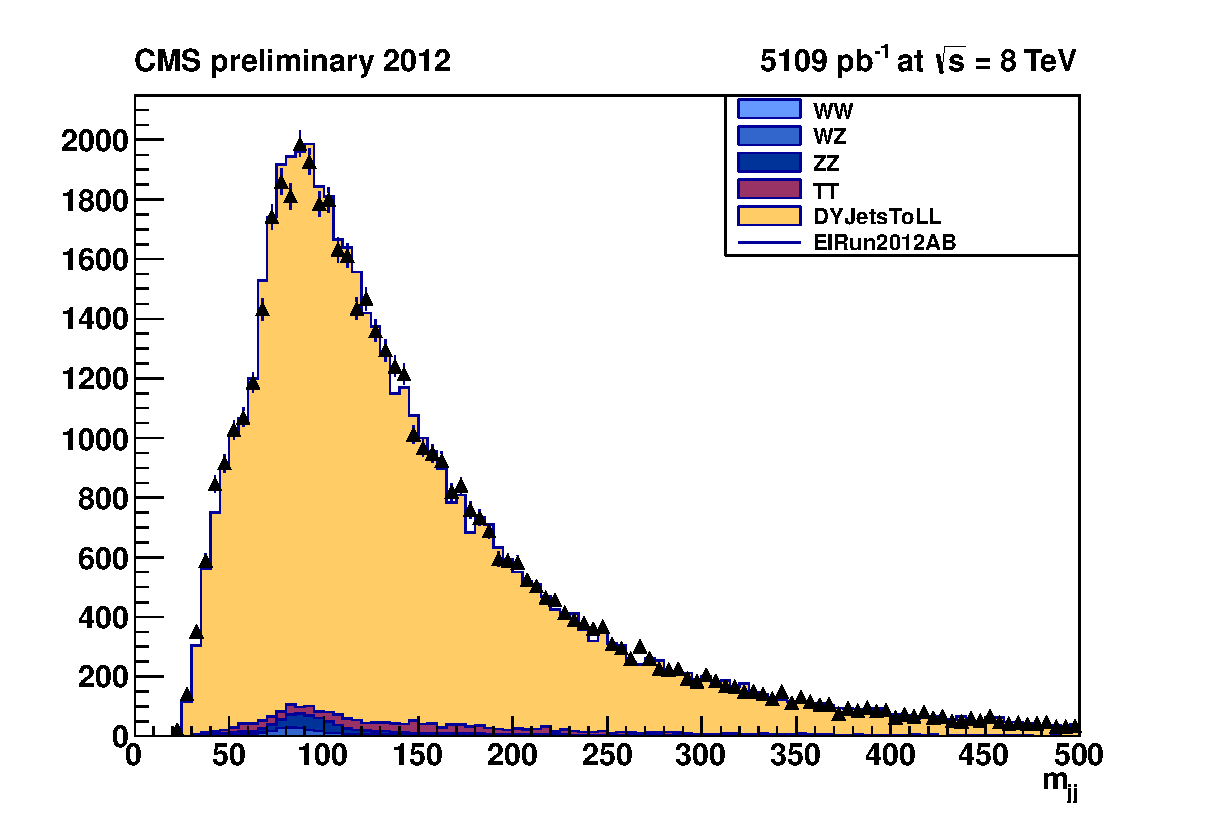
\includegraphics[width=0.5\textwidth]{images/zjjmass_ElRun2012.eps}
 % 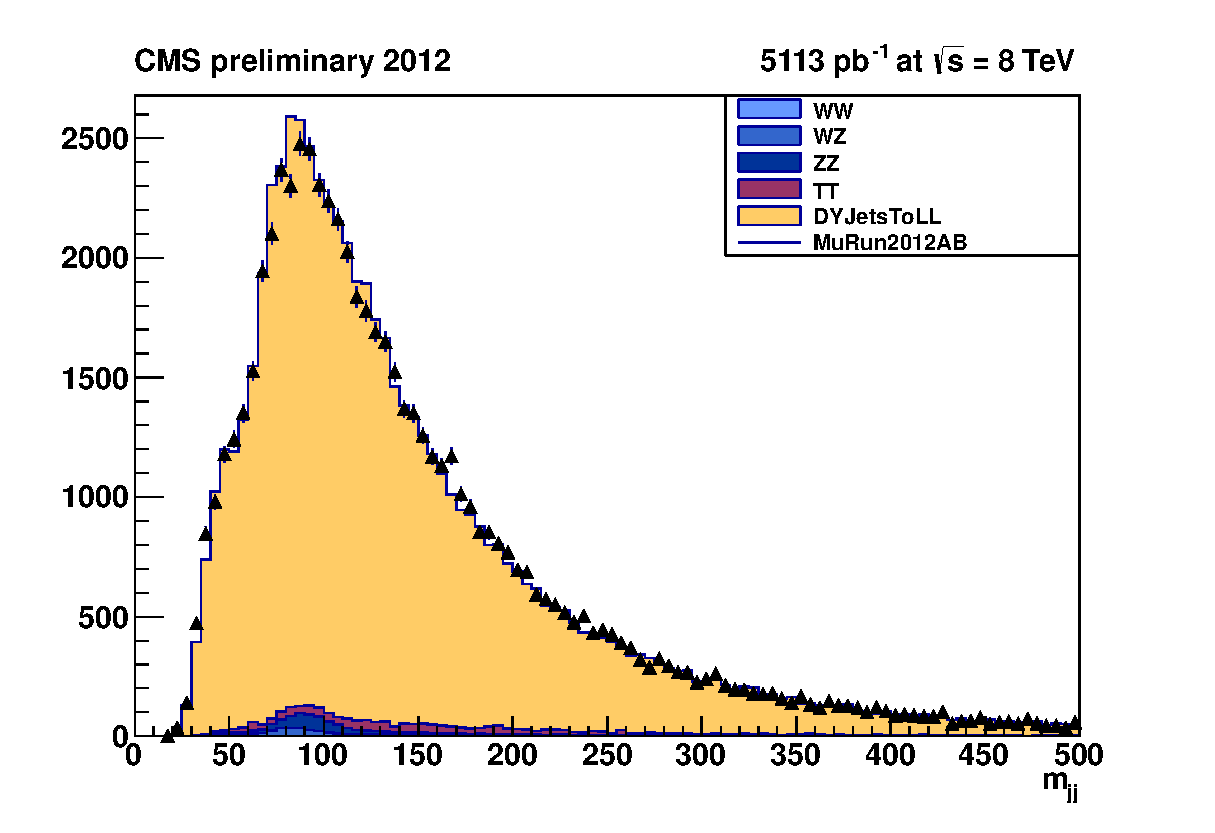
\includegraphics[width=0.5\textwidth]{images/zjjmass_MuRun2012.eps}
  \begin{center}
    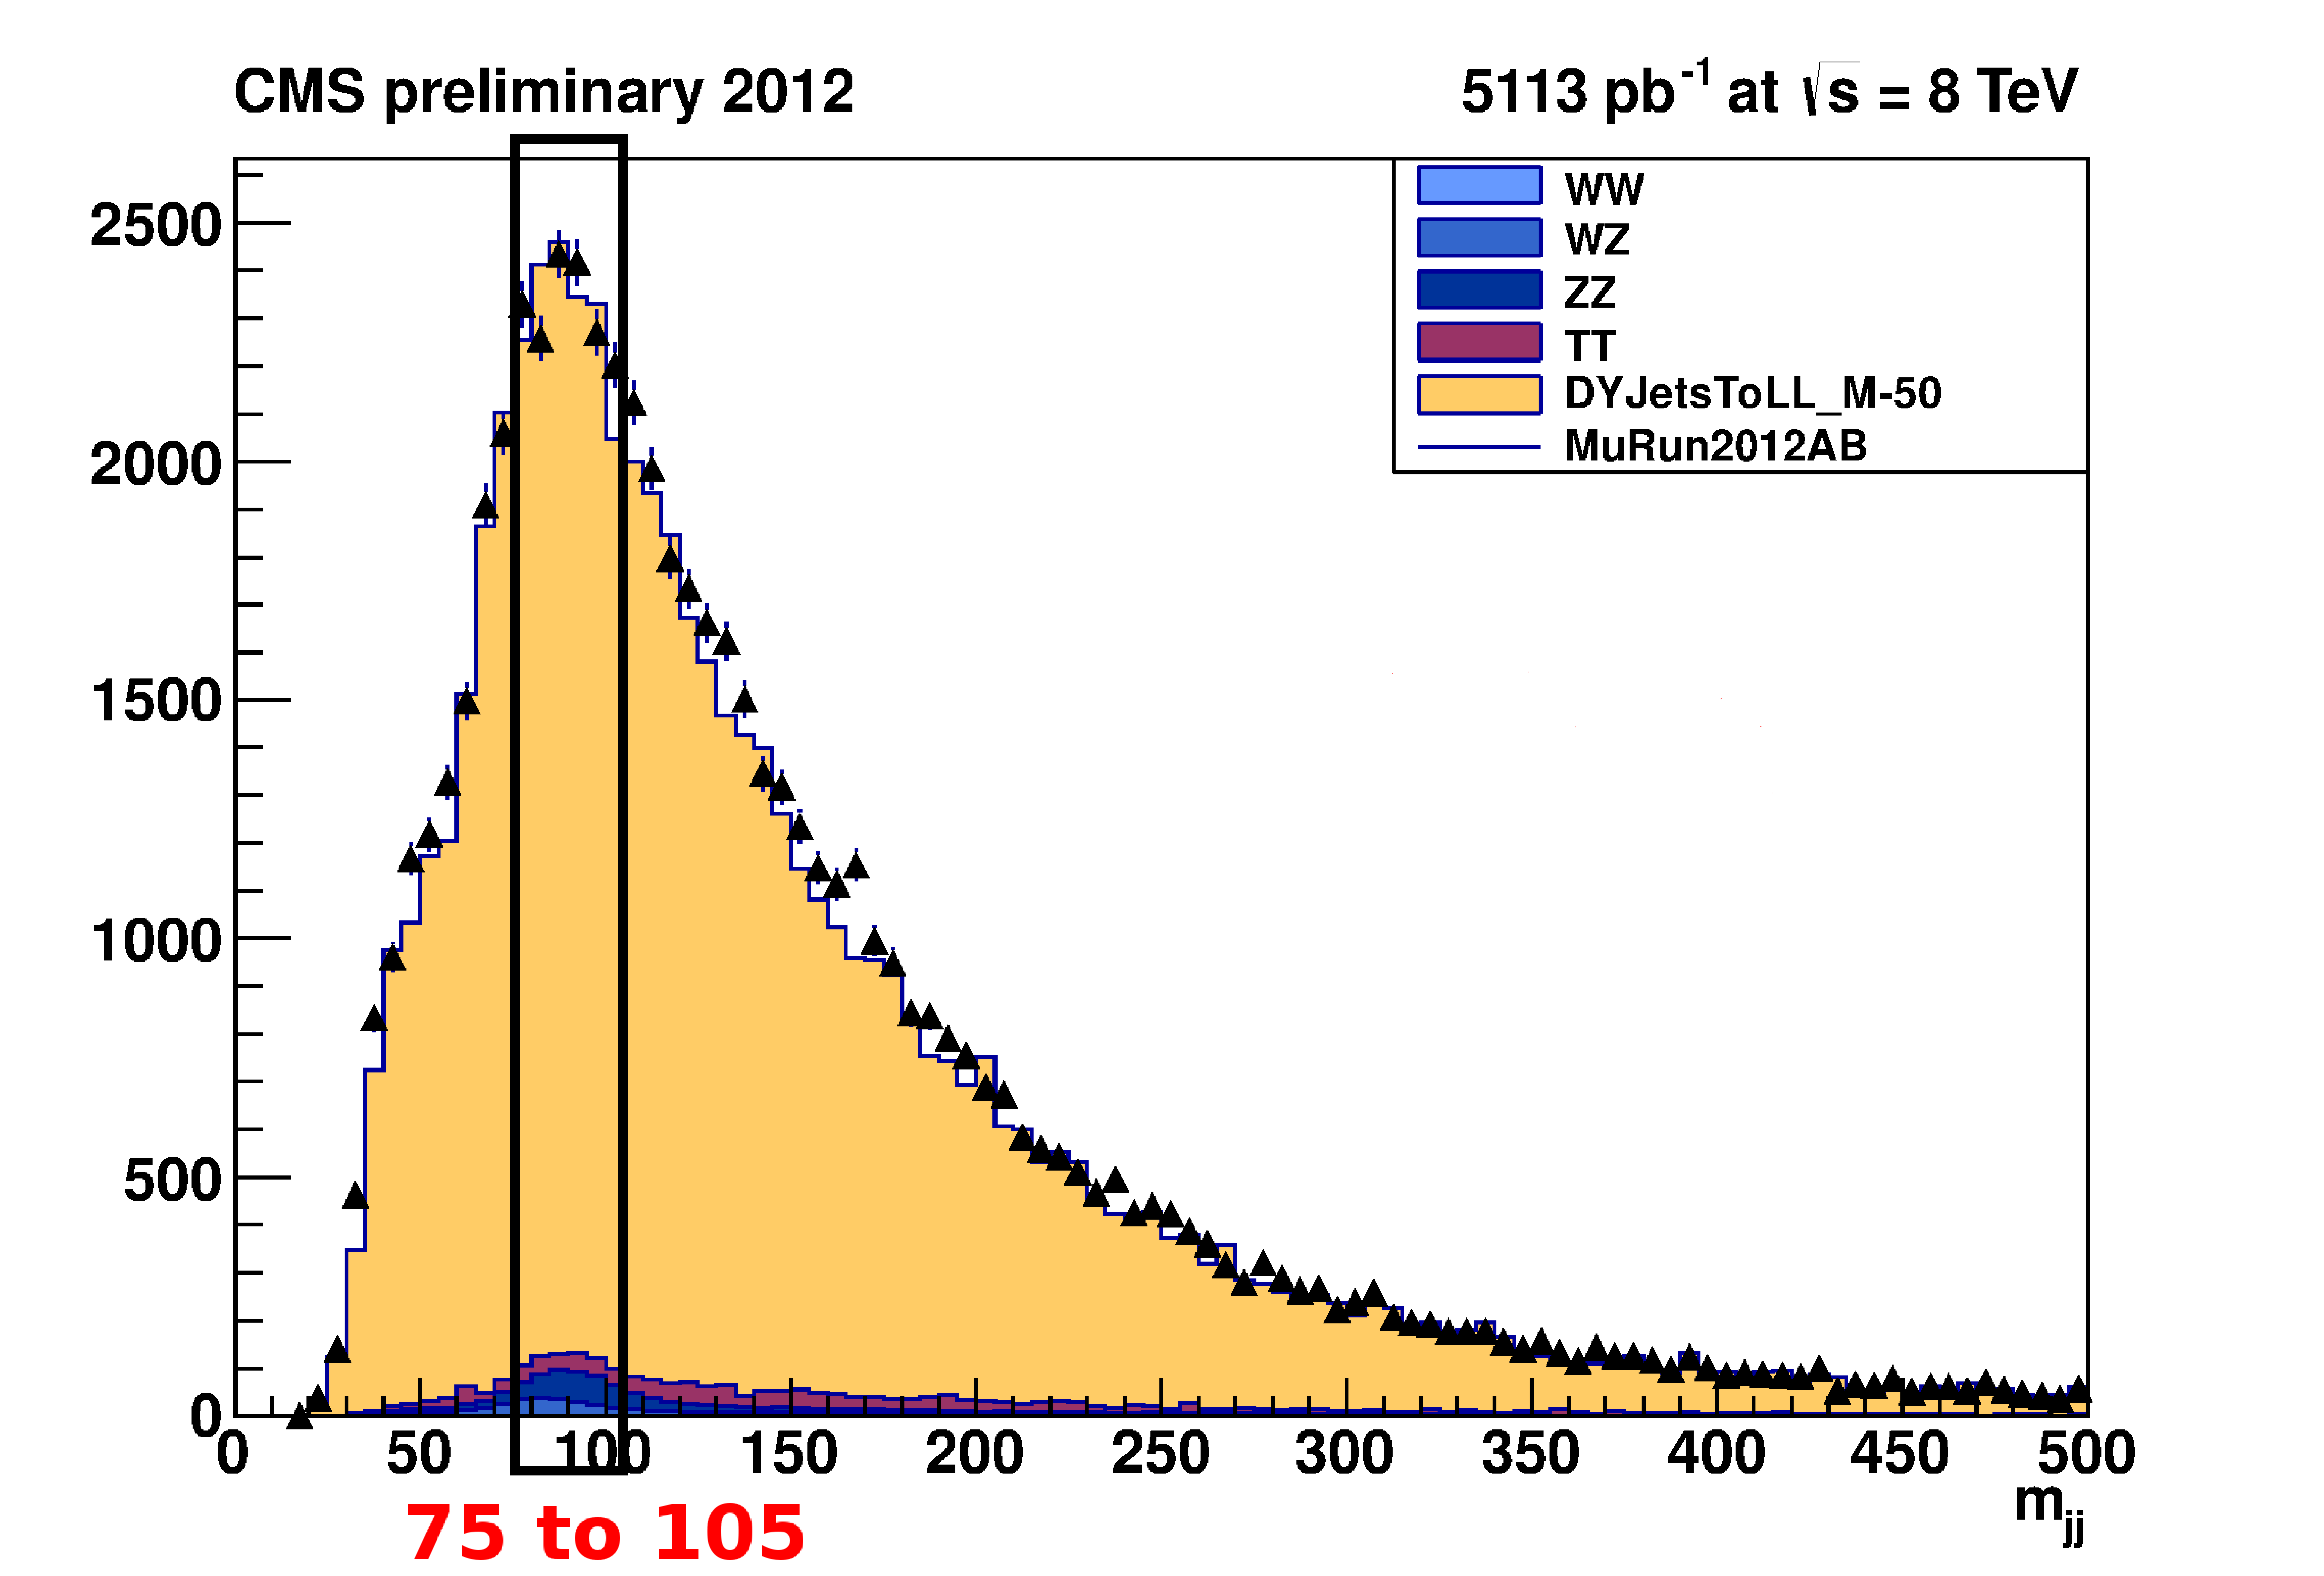
\includegraphics[width=0.6\textwidth]{images/zjjmass_MuRun2012_blind.eps}
  \end{center}

 % \begin{columns}
 %   \begin{column}{0.4\textwidth}
 %      \begin{block}{}
 %       \begin{center}
 %         All plots are either inclusive pre-selection or are in the sidebands.\\
 %        \end{center}
 %     \end{block}
 %   \end{column}
 %    \begin{column}{0.6\textwidth}
 %     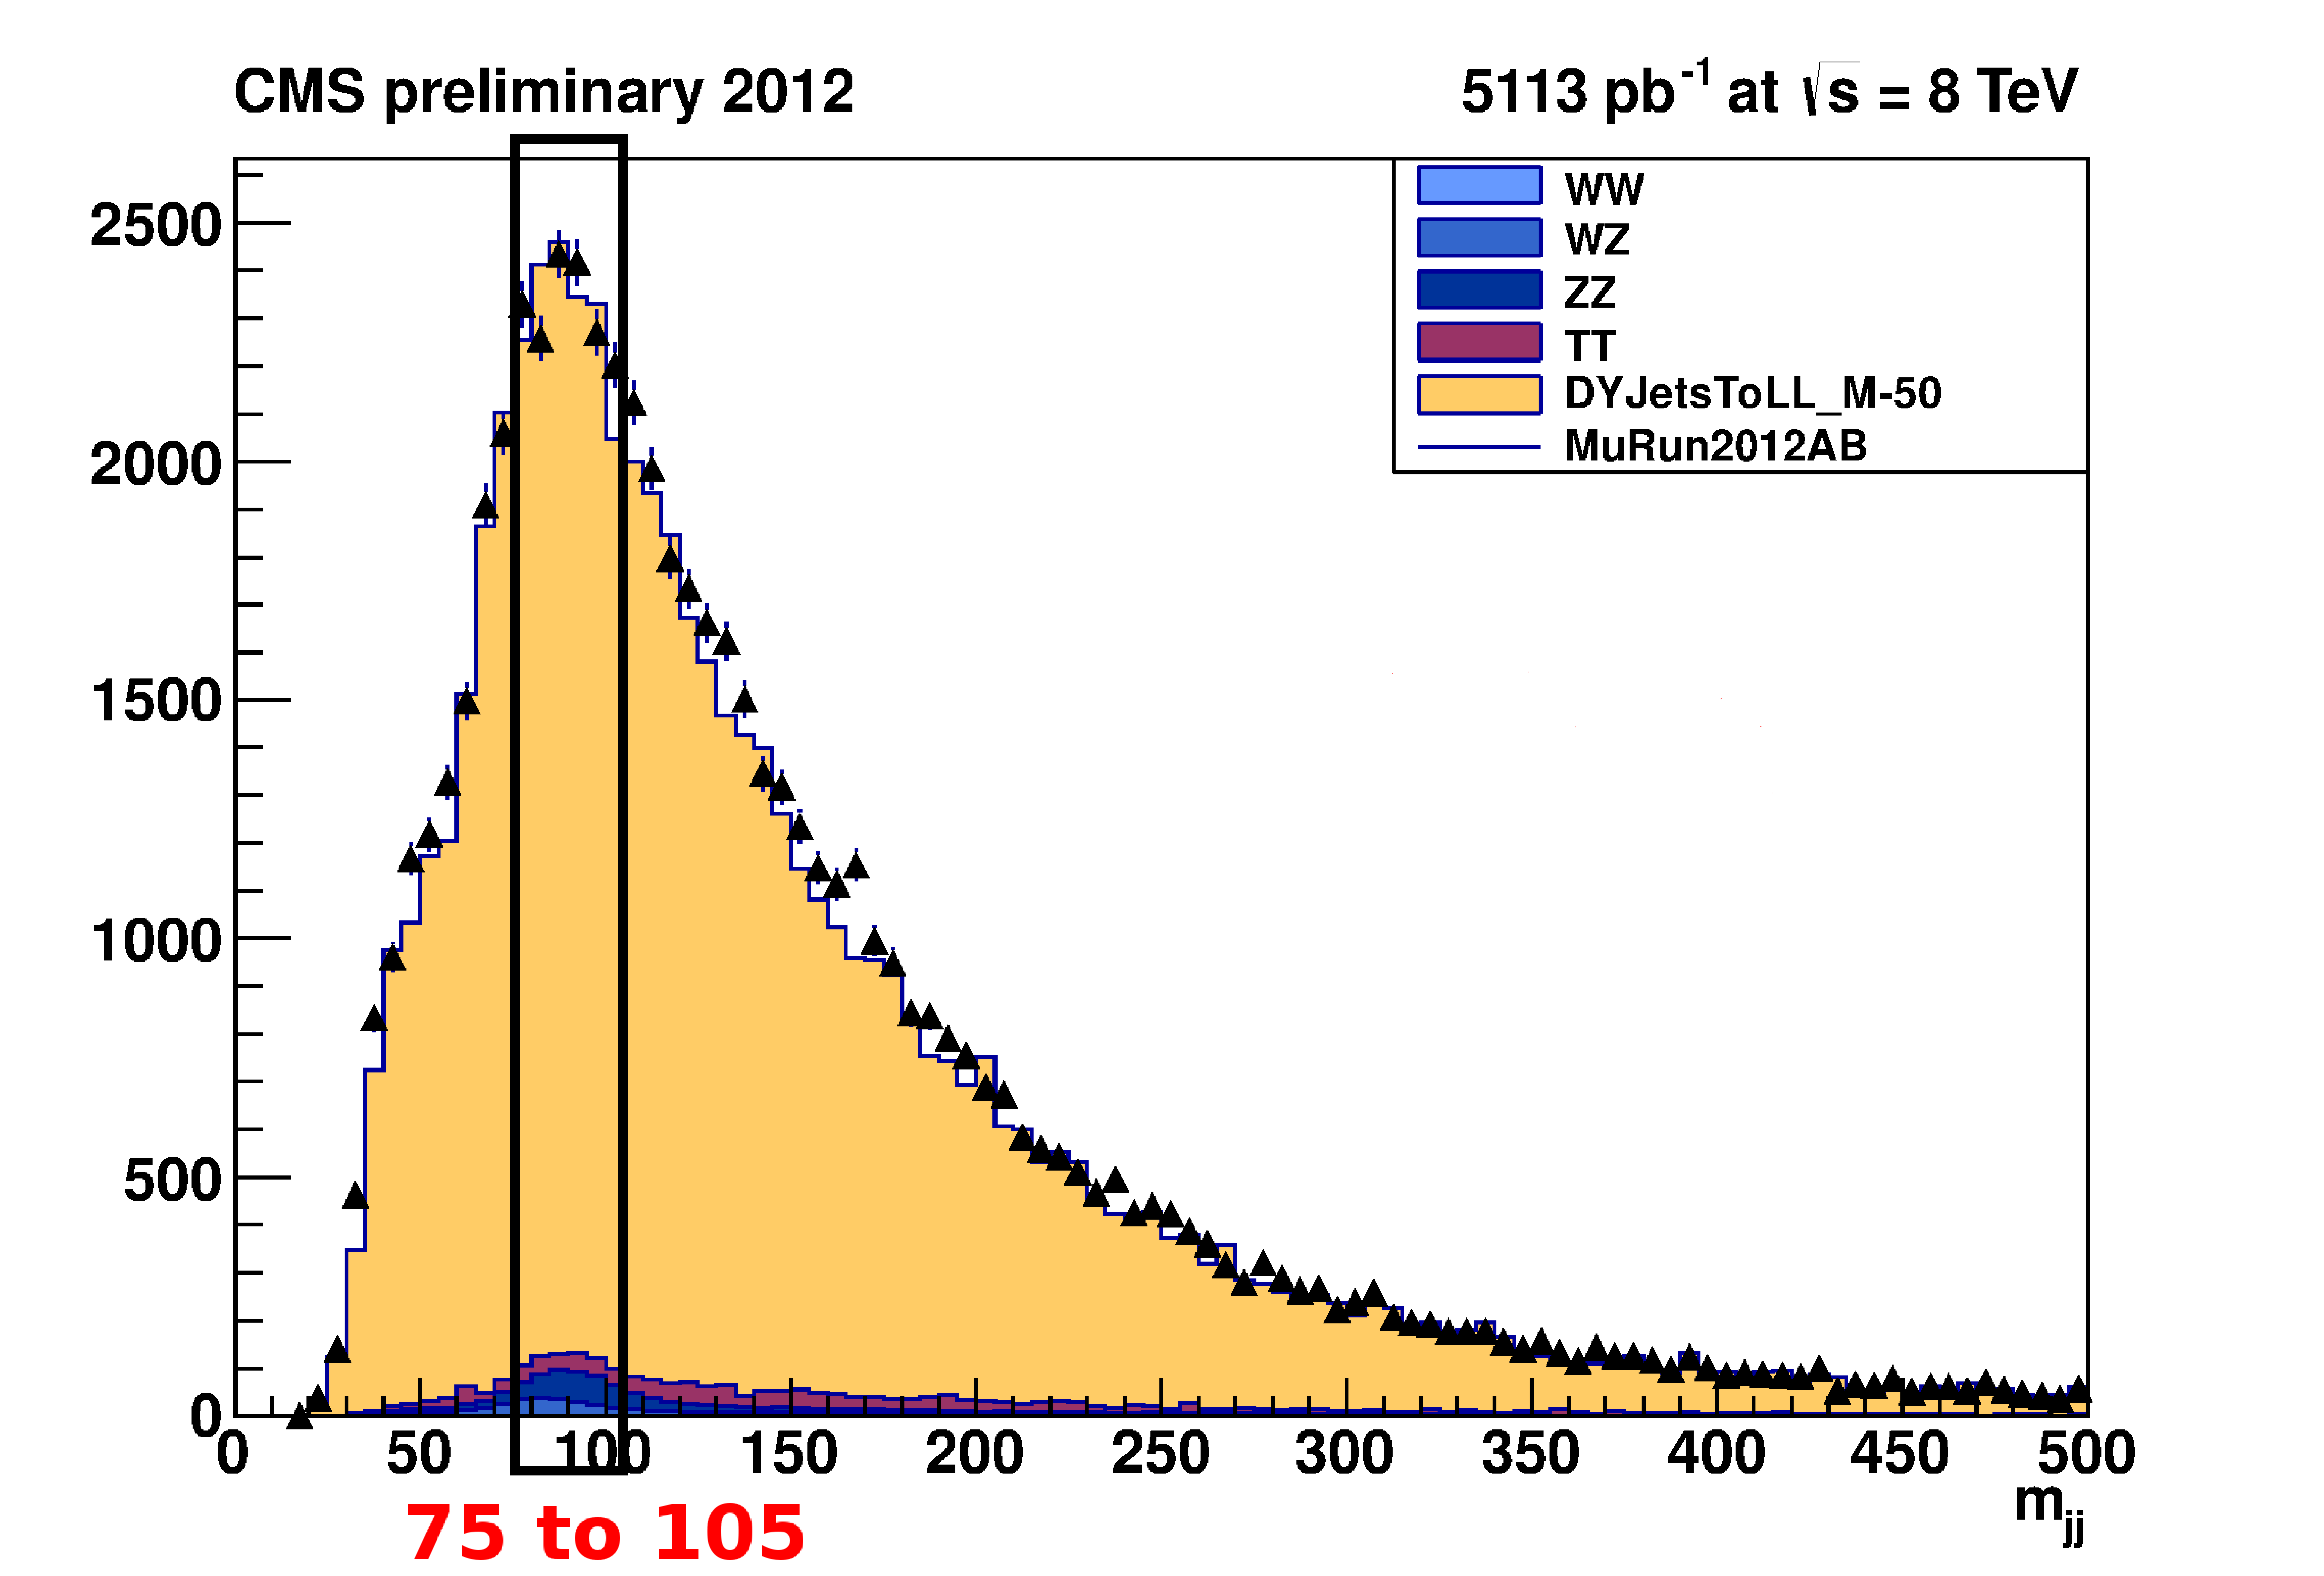
\includegraphics[width=0.9\textwidth]{images/zjjmass_MuRun2012_blind.eps}
 %    \end{column}
 % \end{columns}
  
\end{frame}

%\begin{frame}{Data-MC plots Pretag}
%  \begin{center}
%    Electrons\\
%    $\phi$ \hspace{7.5em} $\phi^{*}$ \hspace{7.5em} Helicity LD
%    \\
%  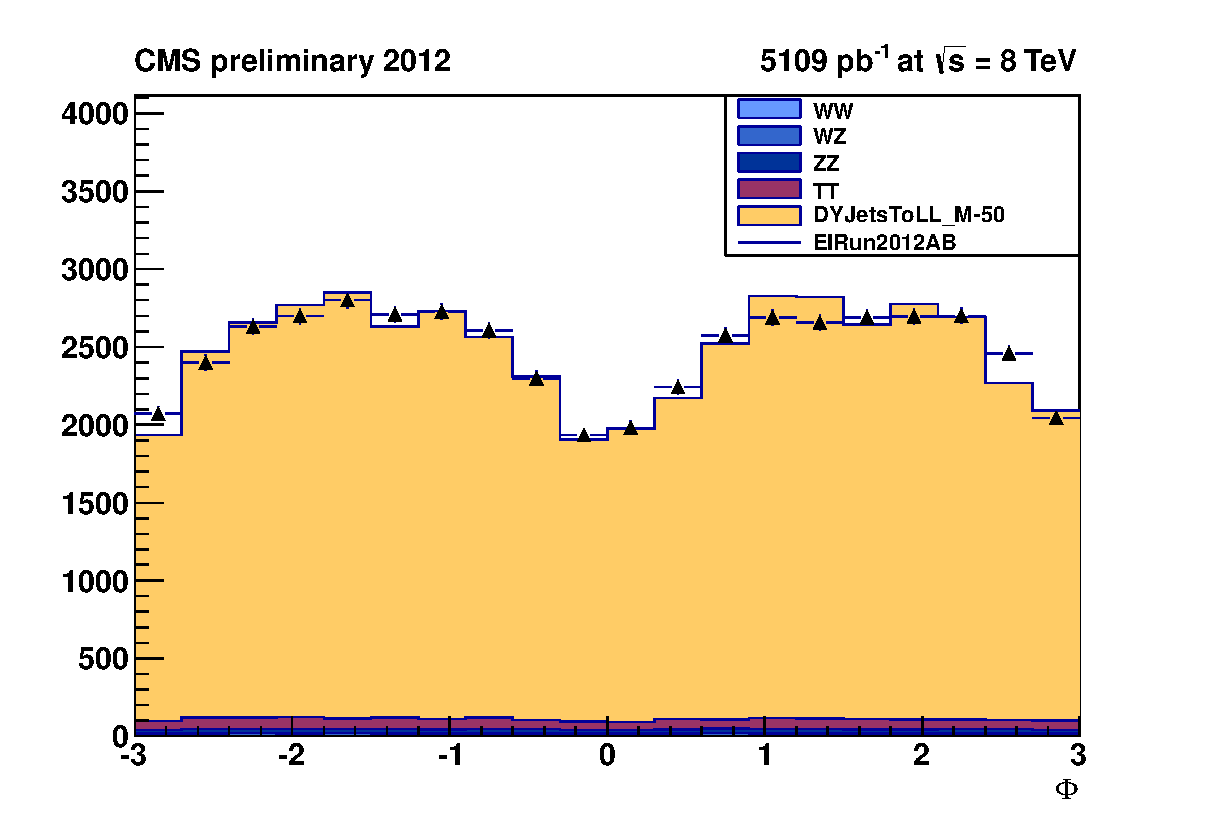
\includegraphics[width=0.33\textwidth]{images/phiRefit_ElRun2012.eps}
%  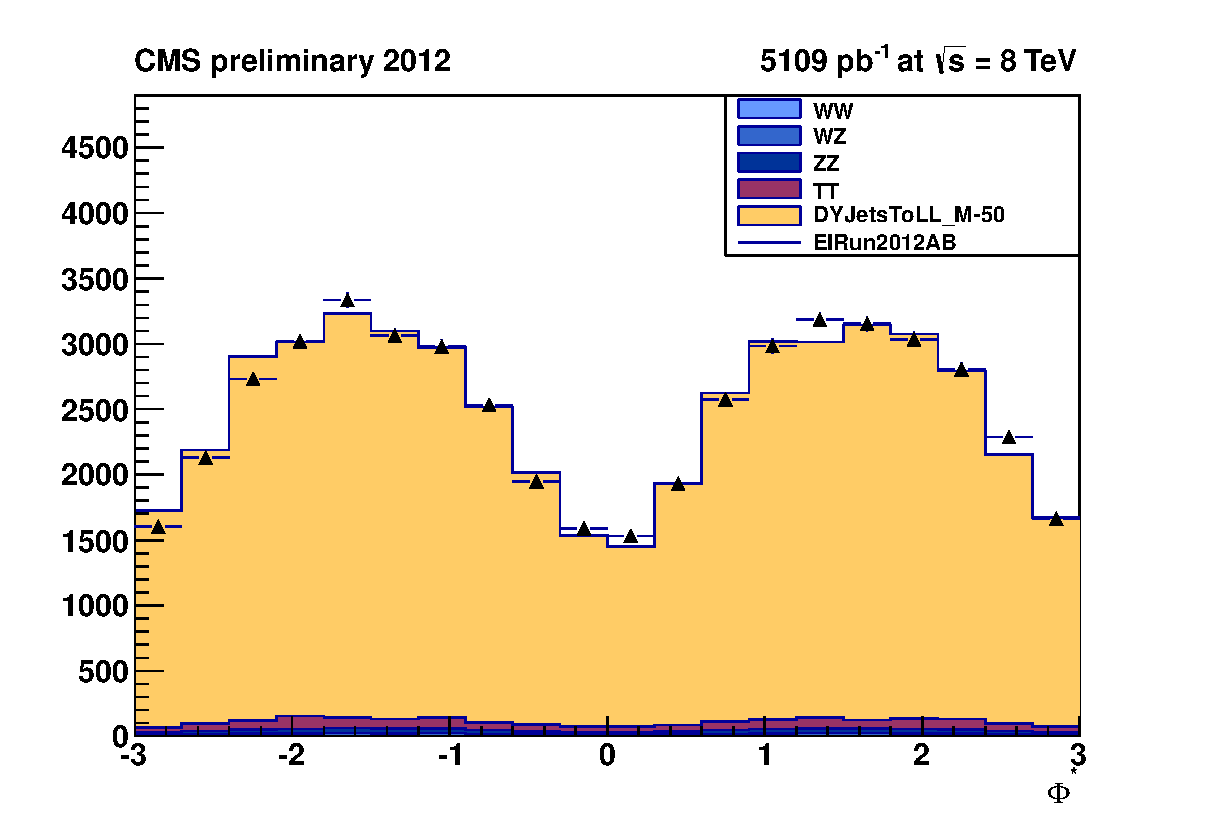
\includegraphics[width=0.33\textwidth]{images/phiStarRefit_ElRun2012.eps}
%  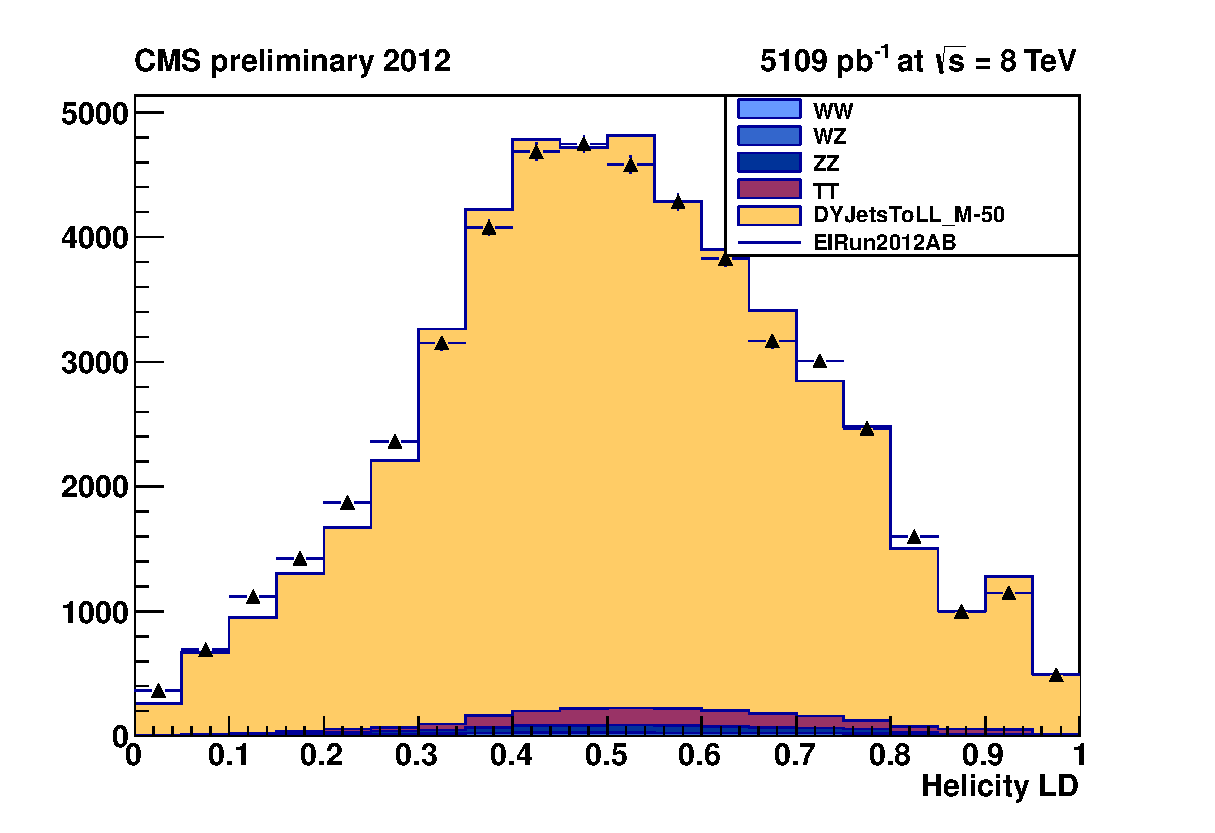
\includegraphics[width=0.33\textwidth]{images/HelyLDRefit_ElRun2012.eps}\\
%  $cos\theta_{1}$ \hspace{7.5em} $cos\theta_{1}^{*}$ \hspace{7.5em} $cos\theta_{2}$
%  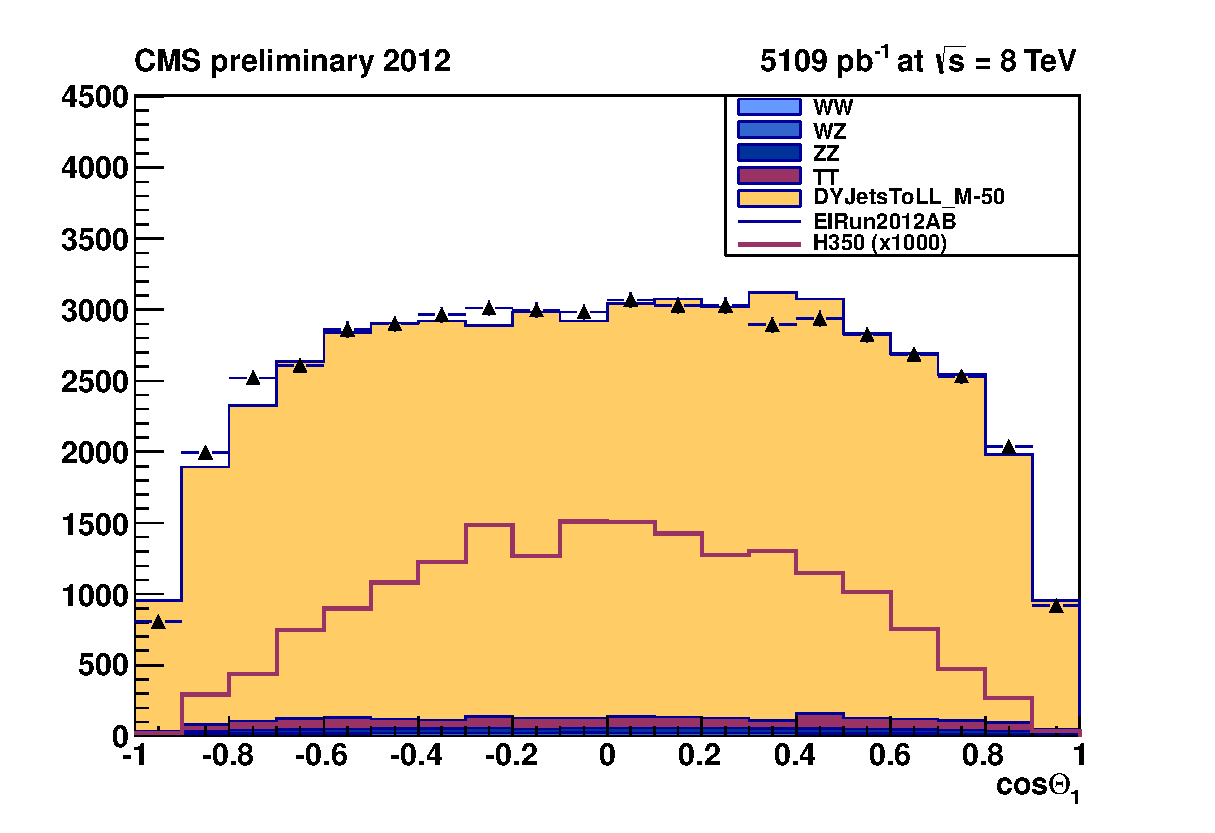
\includegraphics[width=0.33\textwidth]{images/cosTheta1Refit_ElRun2012.eps}
%  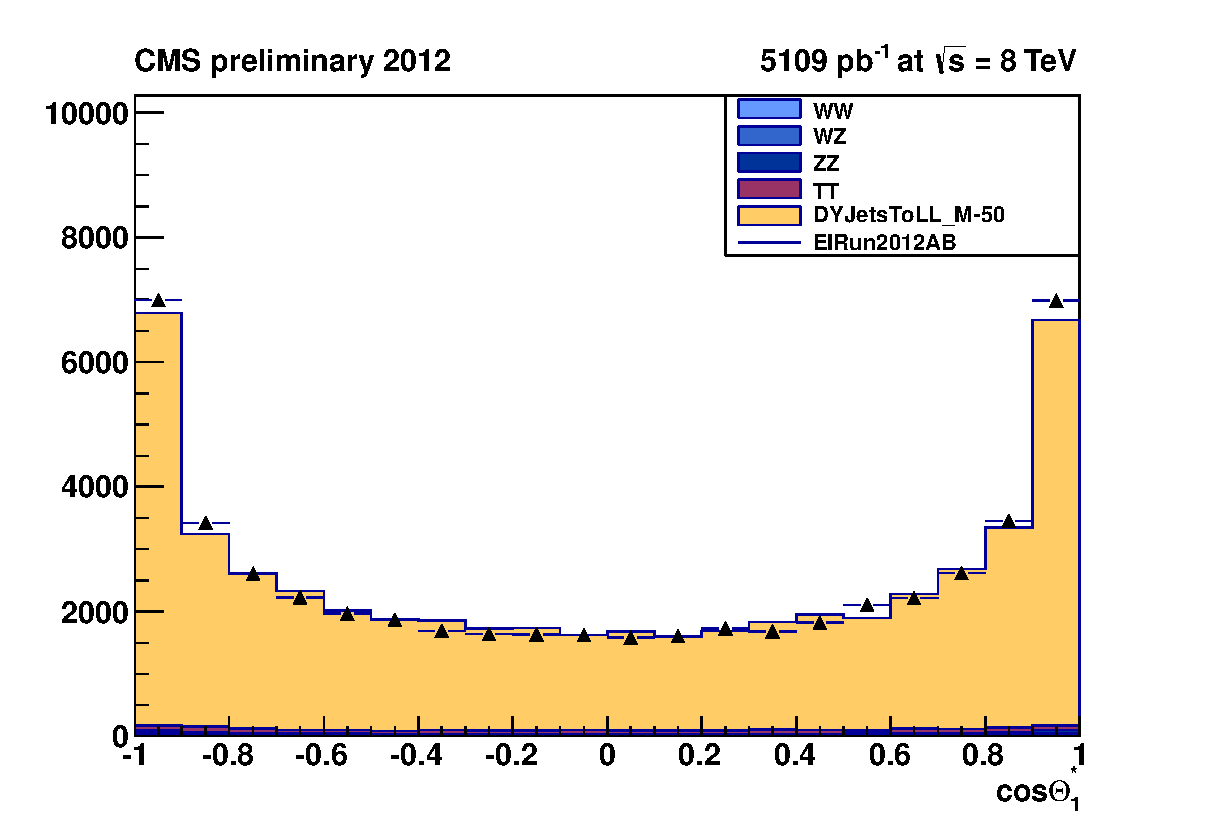
\includegraphics[width=0.33\textwidth]{images/cosTheta1StarRefit_ElRun2012.eps}
%  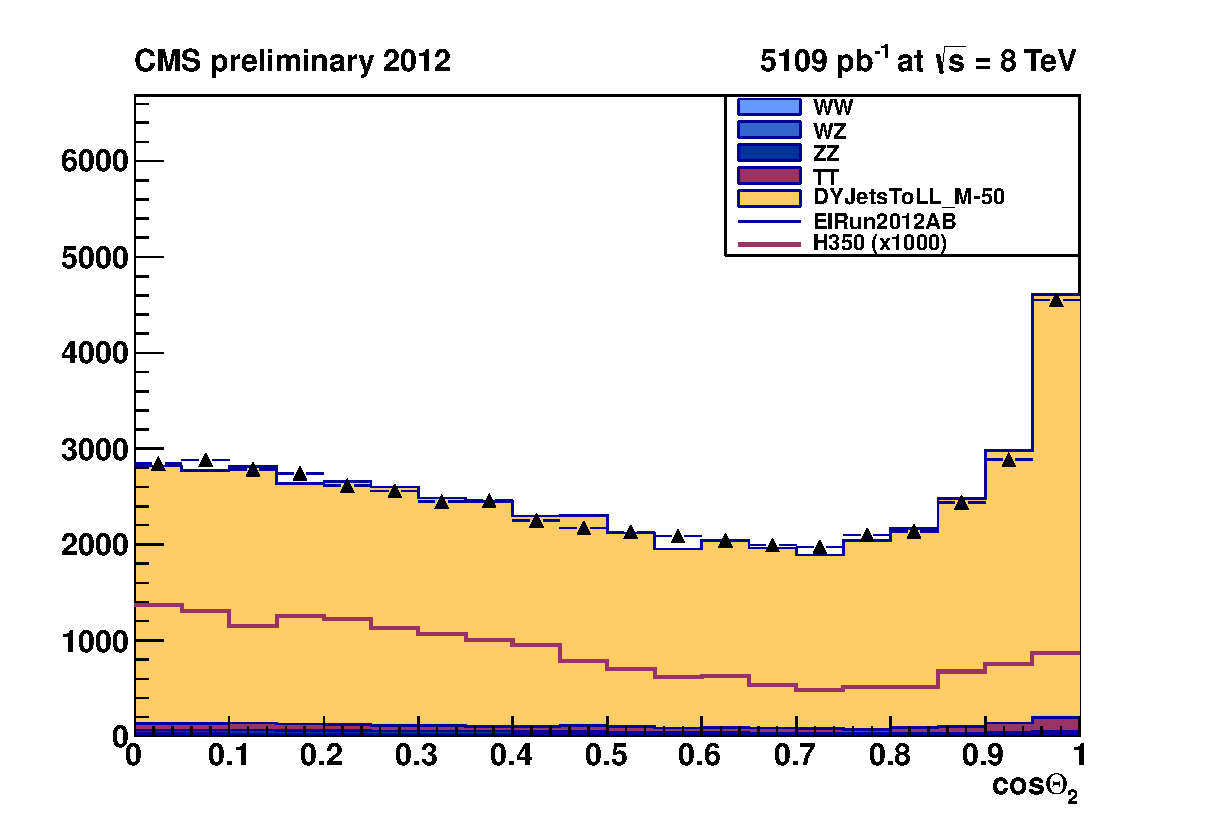
\includegraphics[width=0.33\textwidth]{images/cosTheta2Refit_ElRun2012.eps}
%  \end{center}
%\end{frame}



%\begin{frame}{Data-MC plots Pretag}
%  \begin{center}
%    Muons\\
%    $\phi$ \hspace{7.5em} $\phi^{*}$ \hspace{7.5em} Helicity LD
%    \\
%  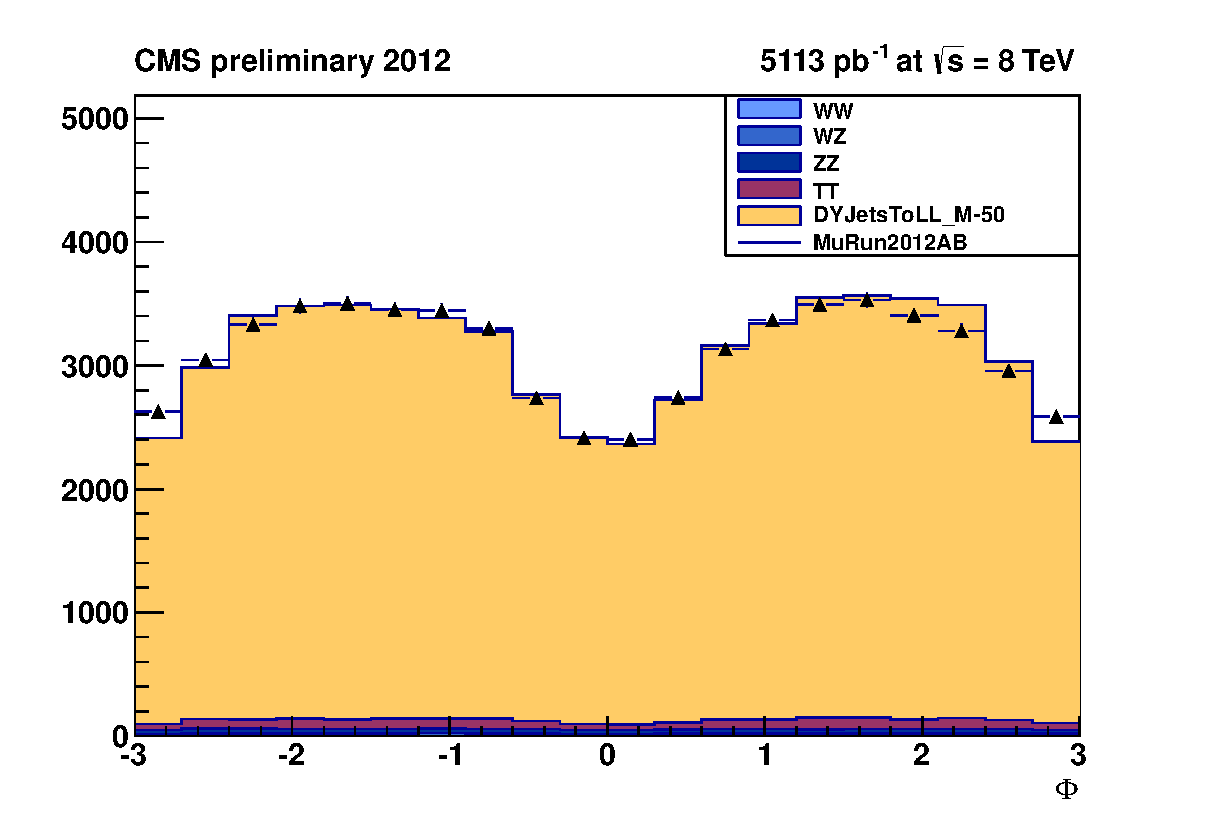
\includegraphics[width=0.33\textwidth]{images/phiRefit_MuRun2012.eps}
%  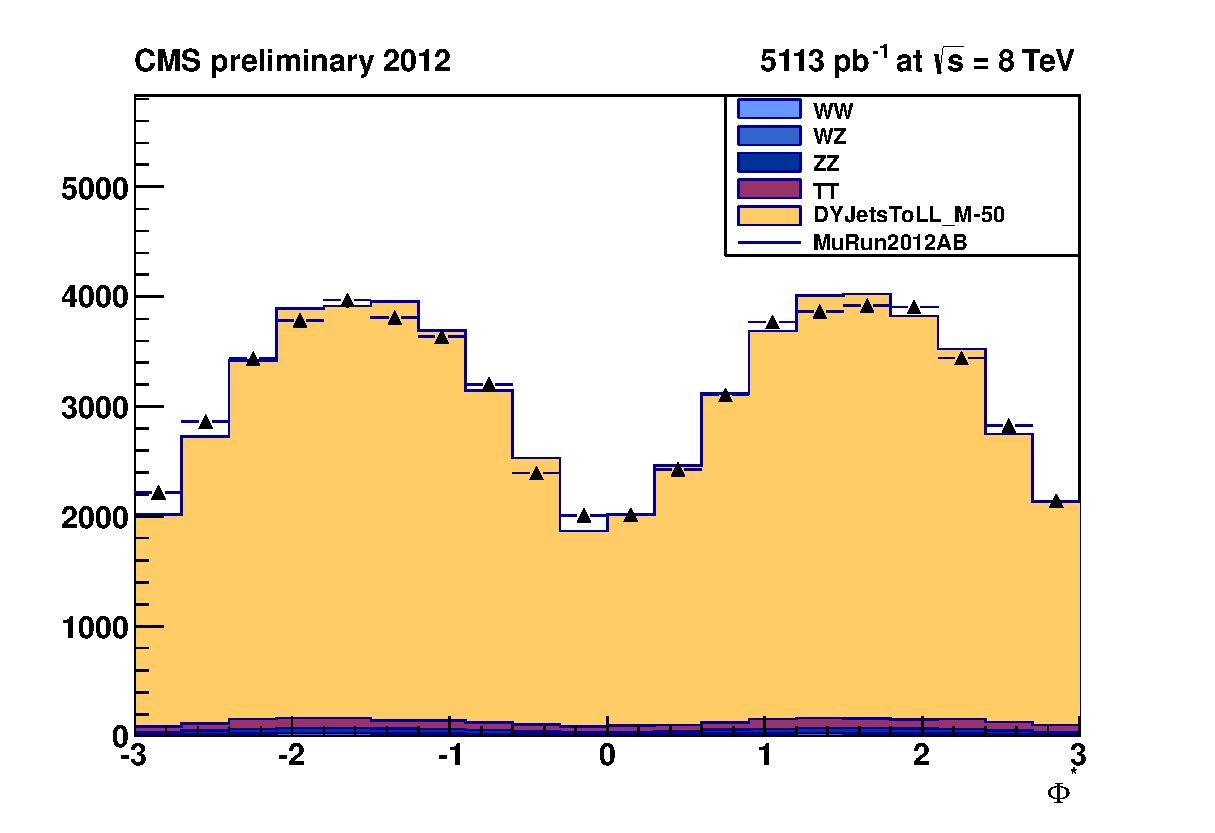
\includegraphics[width=0.33\textwidth]{images/phiStarRefit_MuRun2012.eps}
%  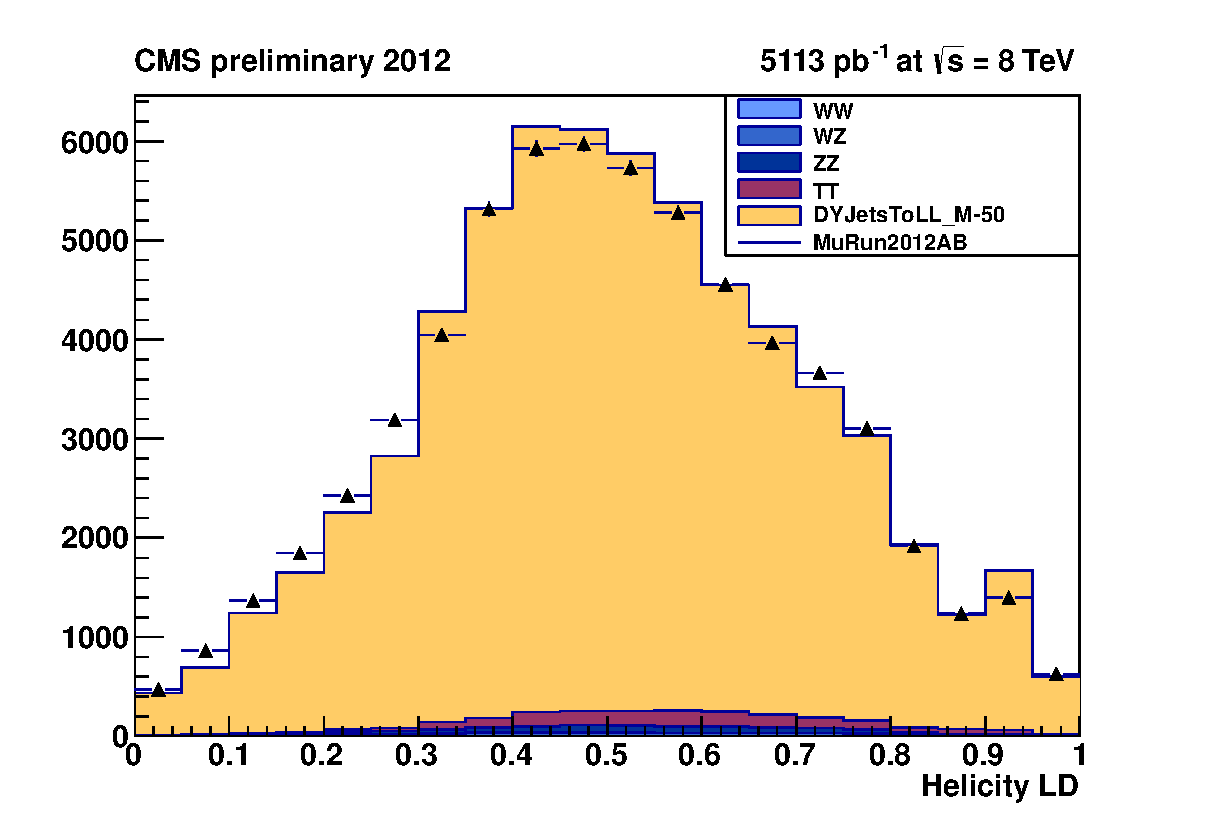
\includegraphics[width=0.33\textwidth]{images/HelyLDRefit_MuRun2012.eps}\\
%  $cos\theta_{1}$ \hspace{7.5em} $cos\theta_{1}^{*}$ \hspace{7.5em} $cos\theta_{2}$
%  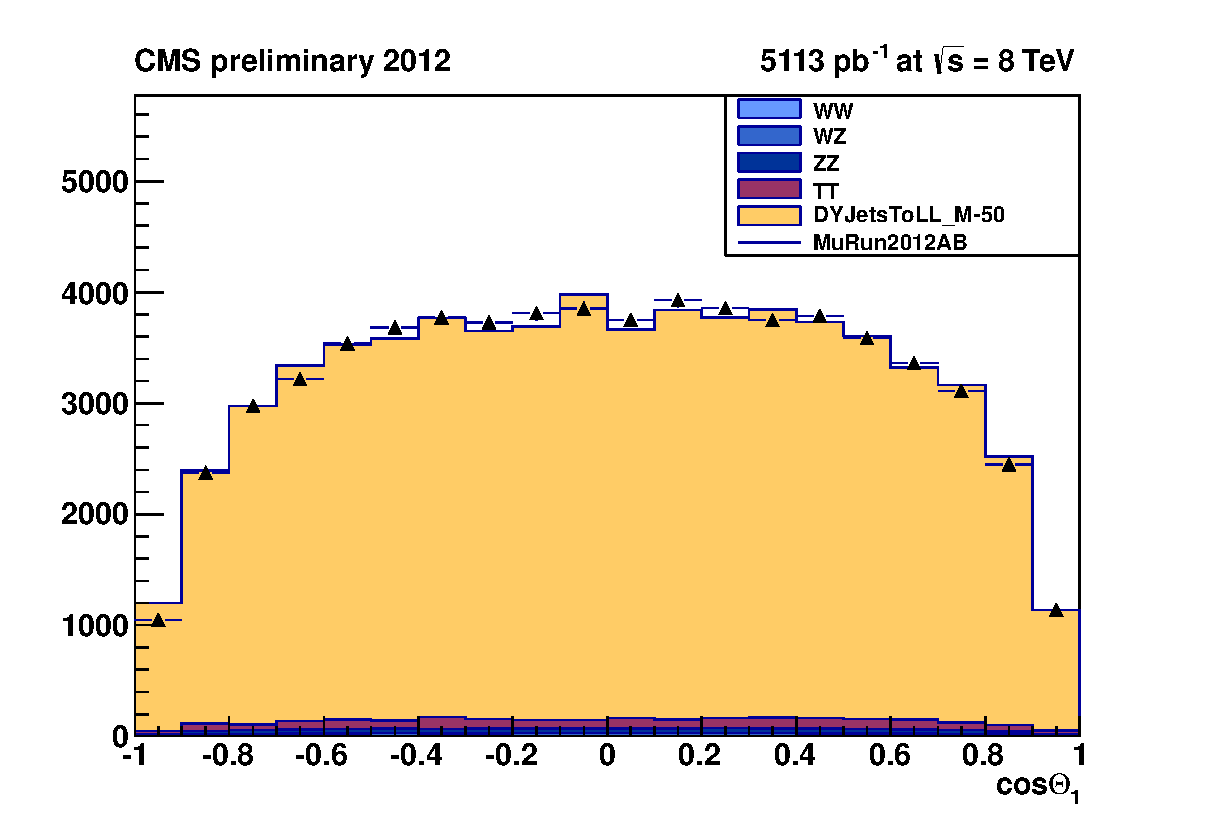
\includegraphics[width=0.33\textwidth]{images/cosTheta1Refit_MuRun2012.eps}
%  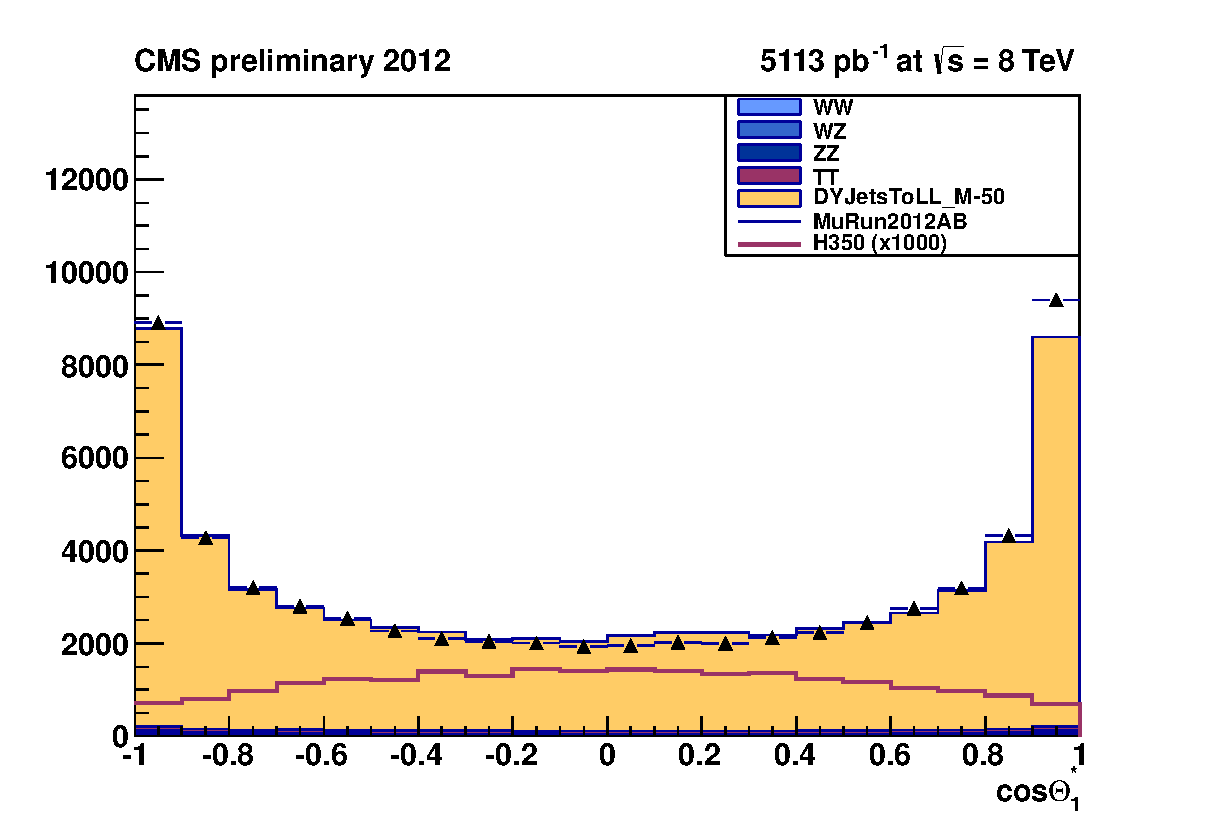
\includegraphics[width=0.33\textwidth]{images/cosTheta1StarRefit_MuRun2012.eps}
%  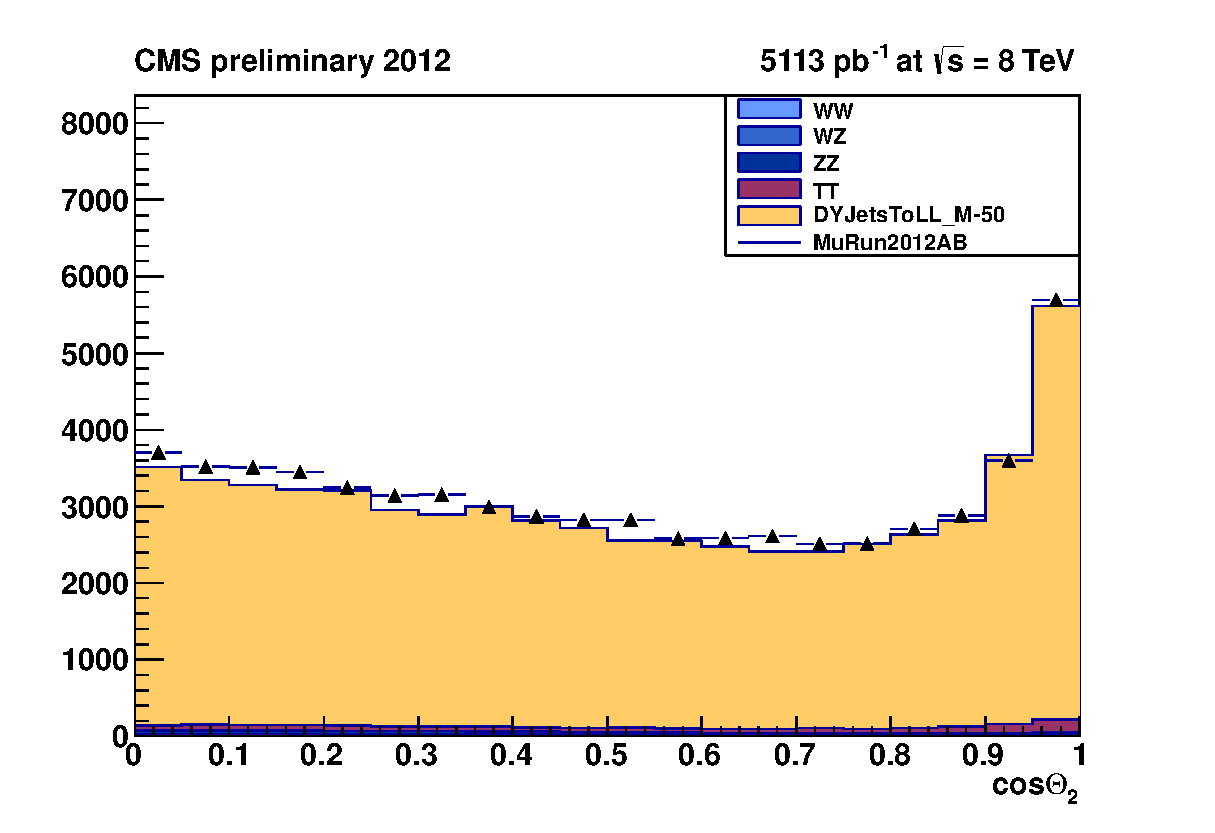
\includegraphics[width=0.33\textwidth]{images/cosTheta2Refit_MuRun2012.eps}
%  \end{center}
%\end{frame}

\begin{frame}{Data-MC $m_{lljj}$ plots - Side Band Region}
  \begin{center}
    Electrons\\
    0-tag \hspace{7.5em} 1-tag \hspace{7.5em} 2-tag
  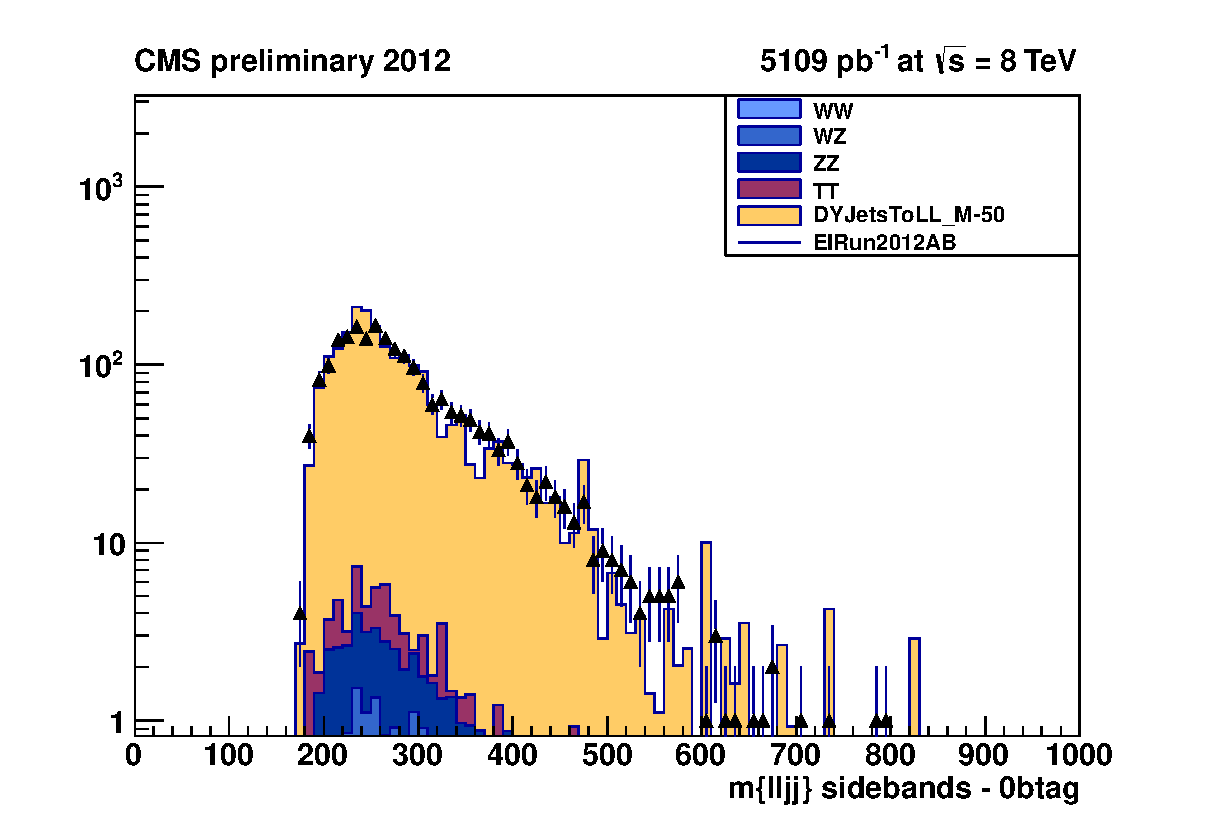
\includegraphics[width=0.33\textwidth]{images/lljjmass_0btagSB_ElRun2012_LOG.eps}
  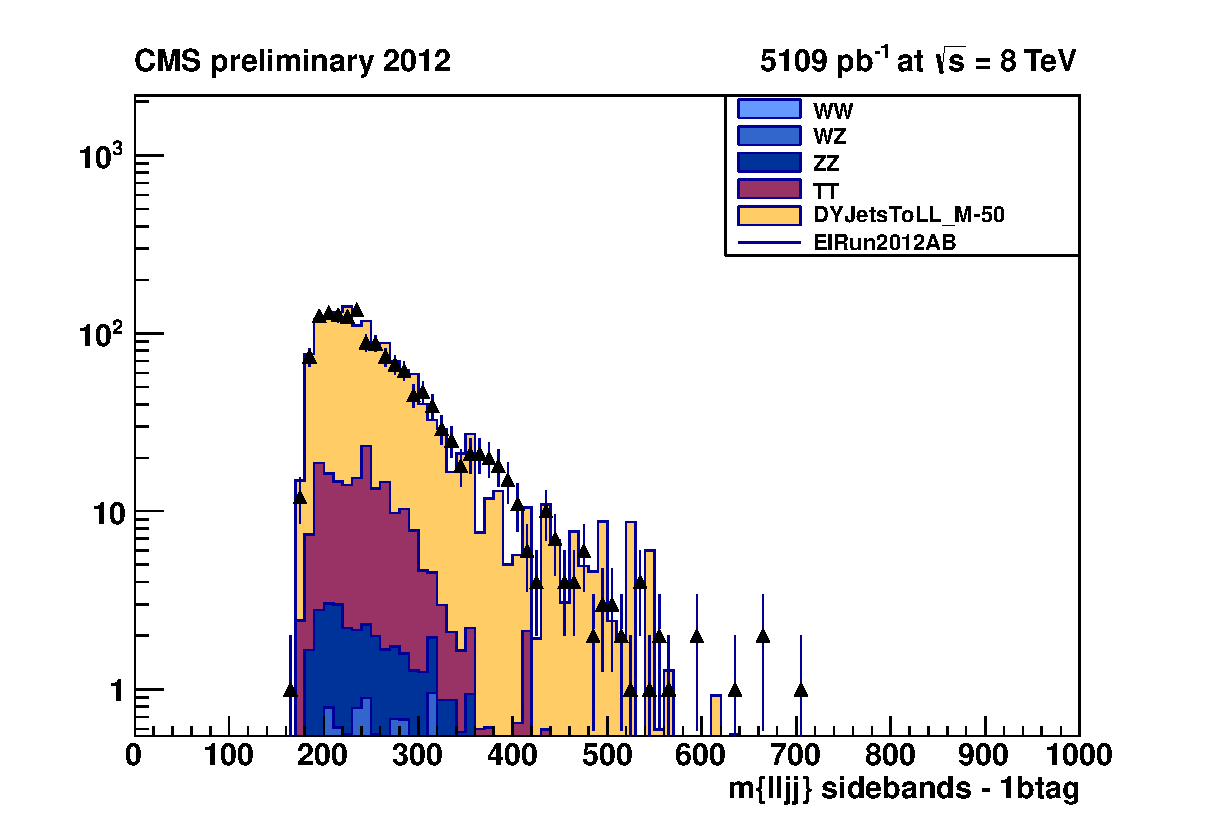
\includegraphics[width=0.33\textwidth]{images/lljjmass_1btagSB_ElRun2012_LOG.eps}
  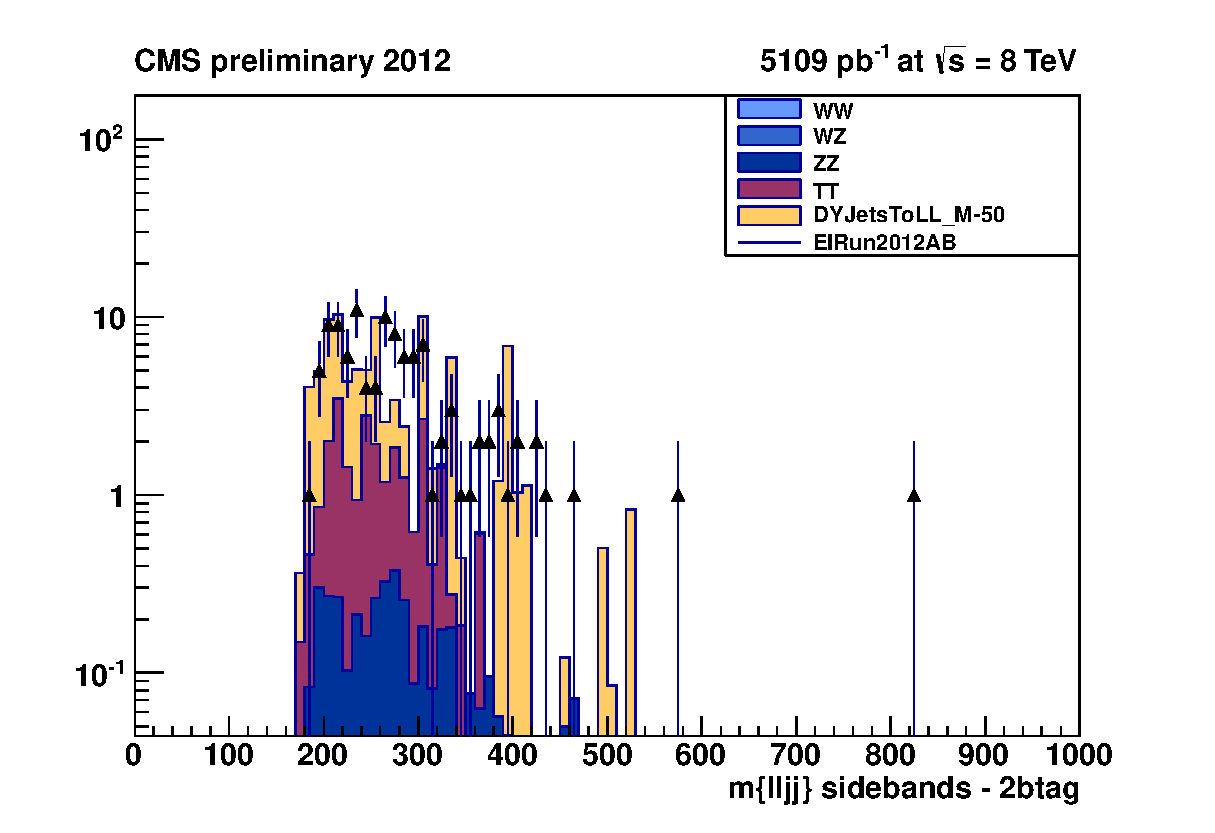
\includegraphics[width=0.33\textwidth]{images/lljjmass_2btagSB_ElRun2012_LOG.eps}\\
  Muons\\
    0-tag \hspace{7.5em} 1-tag \hspace{7.5em} 2-tag
  
  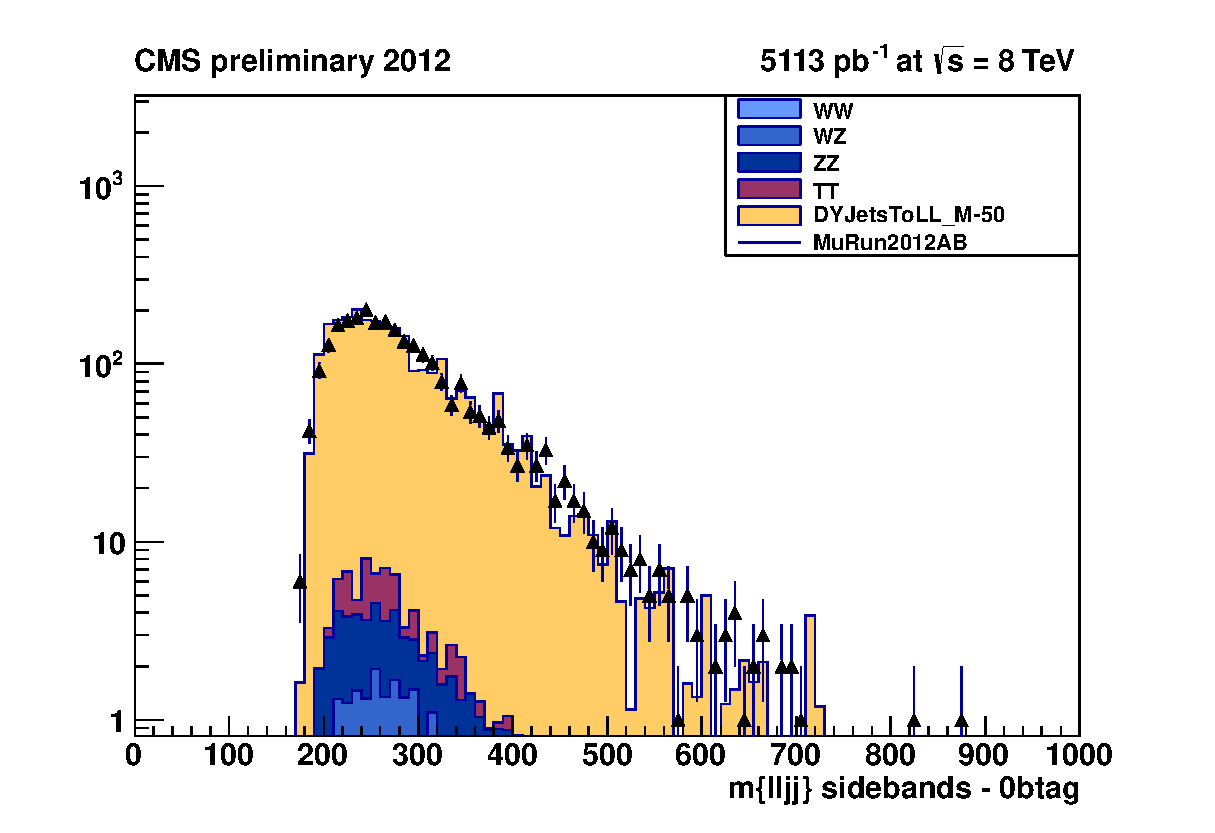
\includegraphics[width=0.33\textwidth]{images/lljjmass_0btagSB_MuRun2012_LOG.eps}
  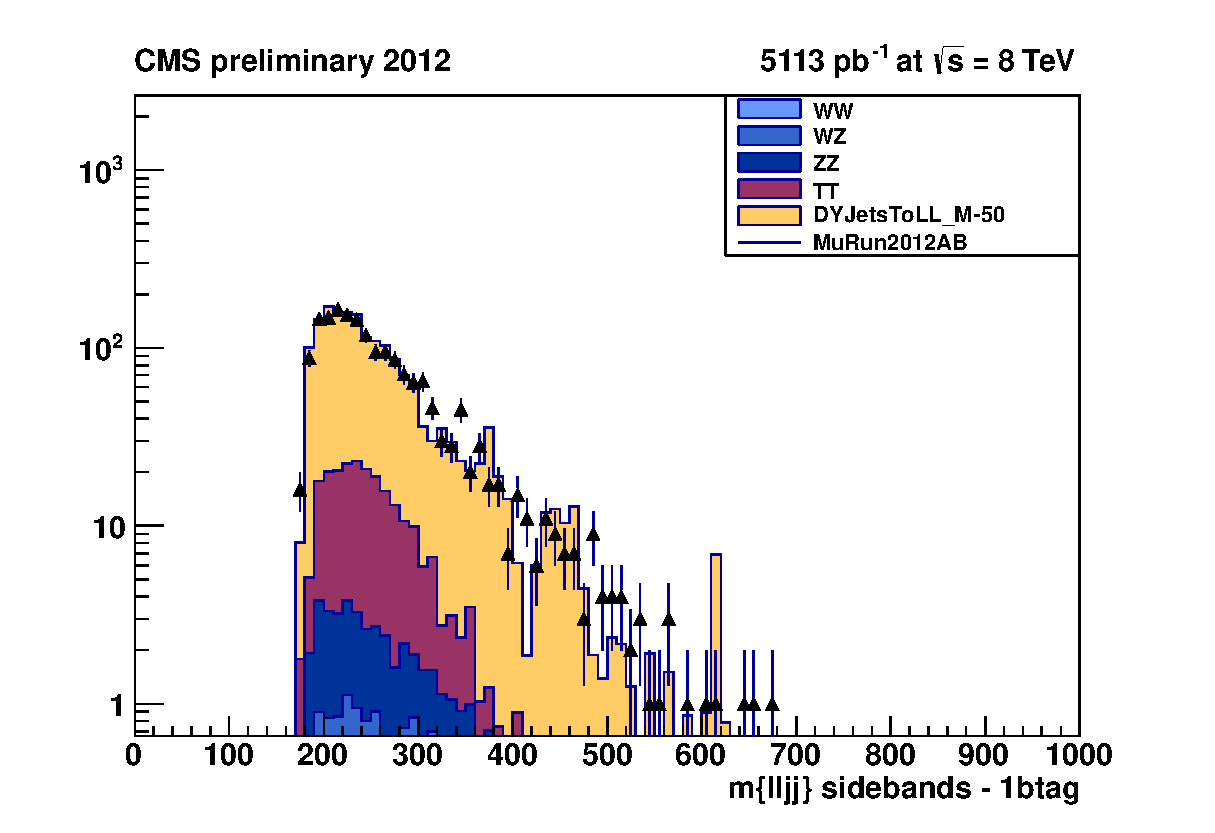
\includegraphics[width=0.33\textwidth]{images/lljjmass_1btagSB_MuRun2012_LOG.eps}
  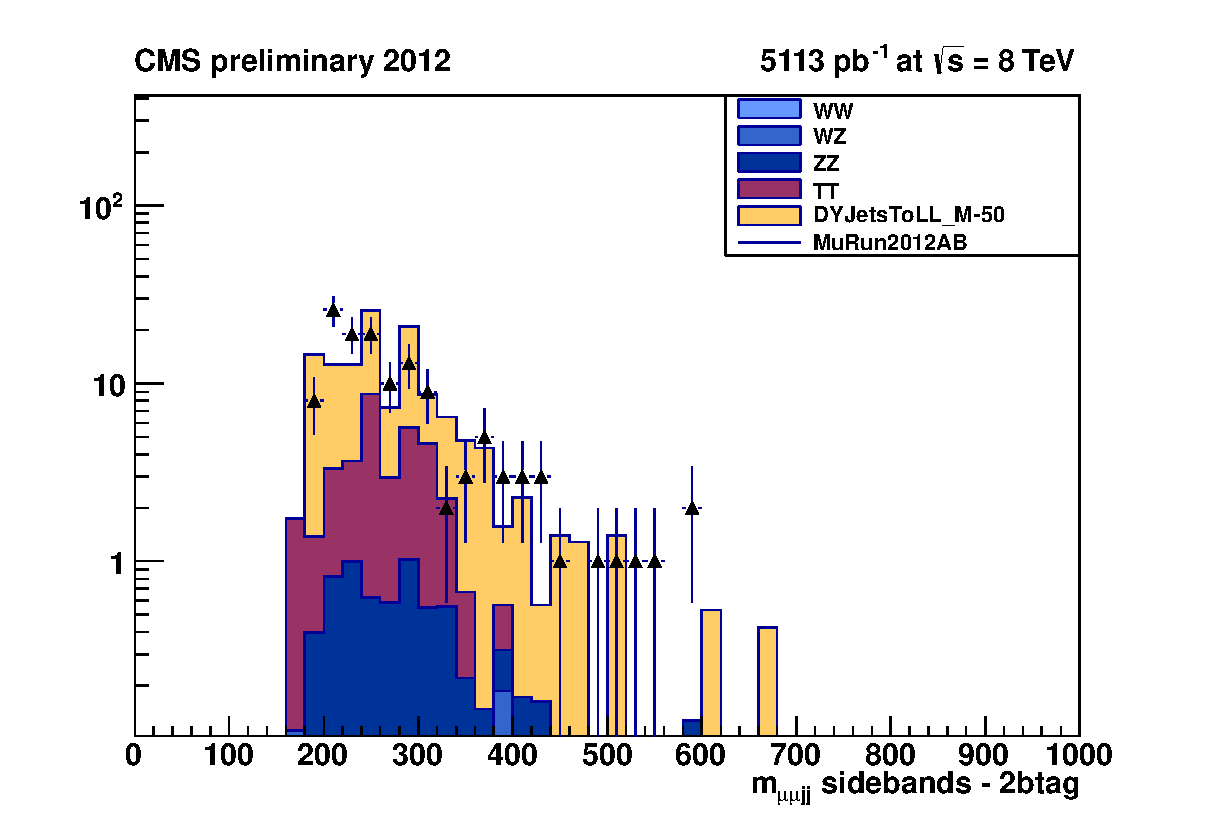
\includegraphics[width=0.33\textwidth]{images/lljjmass_2btagSB_MuRun2012_LOG.eps}
  \end{center}
\end{frame}

%\begin{frame}{$m_{zz}$ Distribution Lineshape Reweighting 2012}
%  \begin{itemize}
%  \item
%    We have the machinery running and are implementing the lineshape reweighting for the 2012 analysis
%  \end{itemize}

%\begin{center}
%  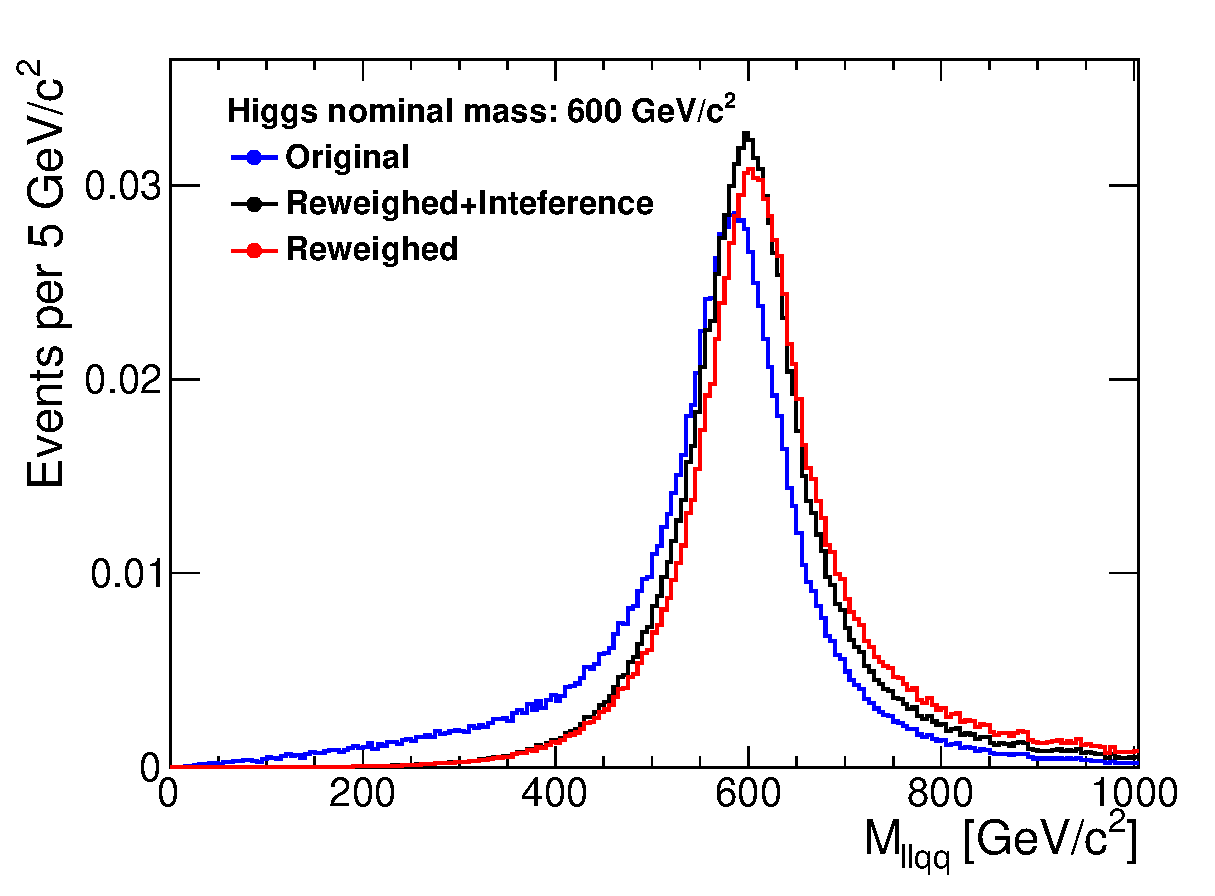
\includegraphics[width=0.7\textwidth]{images/mh600_parton_mother.eps}
%\end{center}
%\end{frame}



\begin{frame}{Background Estimation}
  \scriptsize
  \begin{itemize}
  \item
    We use the mjj sideband in data to get the normalization and a MC shape correction.

 % \begin{block}{}
 %   Number of background events in the signal region extrapolated from 
 % the side band region using the $\alpha(m_{ZZ})$ factor (as a function
 % of m$_{ZZ}$)
 % \begin{equation}
 %   N_{\rm bkg}(m_{ZZ})
 %   =N_{\rm sb}(m_{ZZ})\times\frac{N^{\rm MC}_{\rm bkg}(m_{ZZ})}{N^{\rm MC}_{\rm sb}(m_{ZZ})}
 %   =N_{\rm sb}(m_{ZZ})\times\alpha(m_{ZZ})
 % \end{equation}
 %  \end{block}
\item
  The fit is to a Fermi*CrystallBall function
%  $\alpha$ is a flat factor while we wait for the exclusive samples
\end{itemize}

\begin{center}
%0-tag \vspace{7.5em} 1-tag \vspace{7.5em} 2-tag\\
    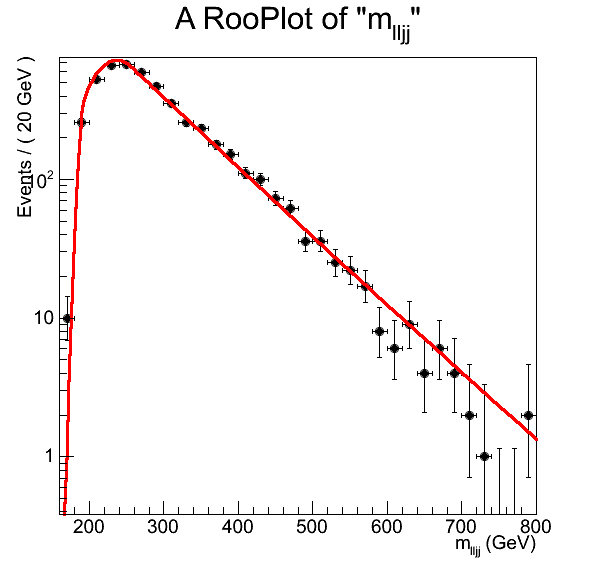
\includegraphics[width=0.3\textwidth]{images/fromDani/mZZ_sidebandsDATA_alpha_0btag_ALL_log.png}
    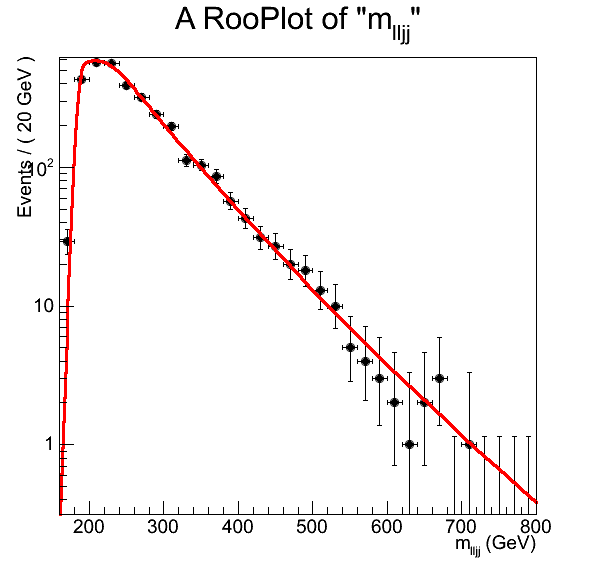
\includegraphics[width=0.3\textwidth]{images/fromDani/mZZ_sidebandsDATA_alpha_1btag_ALL_log.png}
    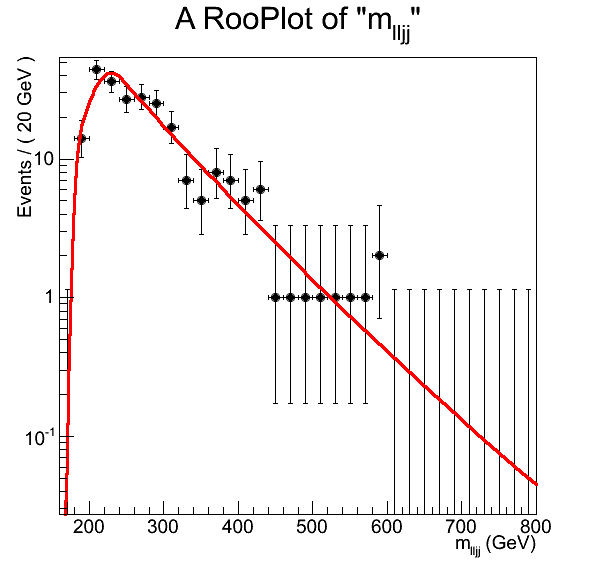
\includegraphics[width=0.3\textwidth]{images/fromDani/mZZ_sidebandsDATA_alpha_2btag_ALL_log.png}\\
0-tag \hspace{10.5em} 1-tag \hspace{10.5em} 2-tag
\end{center}

\end{frame}
